\documentclass[11pt,a4paper]{article}

% ── Encodage & langue ─────────────────────────────────────────────────
\usepackage[utf8]{inputenc}
\usepackage[T1]{fontenc}
\usepackage[french]{babel}

% ── Mise en page ──────────────────────────────────────────────────────
\usepackage[
  top=2.6cm, bottom=2.8cm,
  left=2.4cm, right=2.4cm,
  headheight=16pt
]{geometry}

% ── Typographie ───────────────────────────────────────────────────────
\usepackage{newtxtext,newtxmath}
\usepackage[
  activate={true,nocompatibility},
  final, tracking=true, kerning=true, spacing=true,
  factor=1100, stretch=15, shrink=15
]{microtype}

% ── Couleurs ──────────────────────────────────────────────────────────
\usepackage{xcolor}
\definecolor{primary}{RGB}{13,51,84}
\definecolor{accent}{RGB}{192,65,32}
\definecolor{primarylight}{RGB}{231,238,246}
\definecolor{softbg}{RGB}{247,249,252}
\definecolor{codeframe}{RGB}{205,214,226}
\definecolor{codenumber}{RGB}{148,163,184}
\definecolor{codekw}{RGB}{29,78,152}
\definecolor{codecomment}{RGB}{74,124,80}
\definecolor{darktext}{RGB}{30,41,59}
\definecolor{graytext}{RGB}{100,116,139}
\definecolor{rulecolor}{RGB}{203,213,225}
\definecolor{okgreen}{RGB}{22,101,52}
\definecolor{warnred}{RGB}{154,52,18}

% ── Graphiques & tableaux ─────────────────────────────────────────────
\usepackage{graphicx}
\usepackage{float}
\usepackage{caption}
\usepackage{array,booktabs,multirow,colortbl,longtable,tabularx}

% ── Boîtes & code ─────────────────────────────────────────────────────
\usepackage[skins,breakable]{tcolorbox}
\usepackage{listings}

% ── Liens ─────────────────────────────────────────────────────────────
\usepackage{hyperref}
\hypersetup{
  colorlinks = true,
  linkcolor  = primary,
  urlcolor   = accent,
  citecolor  = primary,
  pdftitle   = {Mini-Projet 2 -- Deploiement et Securisation d'une Infrastructure Reseau d'Entreprise},
  pdfauthor  = {El Gorrim Mohamed, Kchibal Ismail, Junaid Uthman},
}

% ── Listes & en-têtes ─────────────────────────────────────────────────
\usepackage{enumitem}
\usepackage{fancyhdr}
\usepackage{titlesec}
\usepackage{tocloft}

% ─────────────────────────────────────────────────────────────────────
%  CONFIGURATION GLOBALE
% ─────────────────────────────────────────────────────────────────────

\setlength{\parindent}{0pt}
\setlength{\parskip}{0.42em}

\pagestyle{fancy}\fancyhf{}
\fancyhead[L]{\small\color{graytext}\textit{FST Tanger~--~Departement Informatique}}
\fancyhead[R]{\small\color{graytext}\textit{MP2~--~Infrastructure Reseau d'Entreprise}}
\fancyfoot[C]{%
  \footnotesize\color{graytext}%
  \textcolor{rulecolor}{\rule[0.28em]{1.5cm}{0.3pt}}\enspace
  \thepage
  \enspace\textcolor{rulecolor}{\rule[0.28em]{1.5cm}{0.3pt}}}
\renewcommand{\headrulewidth}{0.35pt}
\renewcommand{\footrulewidth}{0pt}

\captionsetup{
  labelfont={bf,color=primary,normalfont},
  textfont={small,color=darktext},
  labelsep=space,
  justification=centering,
  singlelinecheck=false,
  skip=6pt,
  font=small}
\captionsetup[figure]{name=Fig.}
\captionsetup[table]{name=Tab.}

\titleformat{\section}
  {\Large\bfseries\color{primary}}
  {\colorbox{primary}{\textcolor{white}{\,\thesection\,}}}
  {0.75em}{}
  [\vspace{0.28em}{\color{primary!30}\hrule height 1.4pt}]
\titlespacing*{\section}{0pt}{1.8em}{0.8em}

\titleformat{\subsection}
  {\large\bfseries\color{primary!90!black}}
  {\thesubsection}{0.65em}{}
\titlespacing*{\subsection}{0pt}{1.2em}{0.4em}

\titleformat{\subsubsection}
  {\normalsize\bfseries\color{accent}}
  {\thesubsubsection}{0.65em}{}
\titlespacing*{\subsubsection}{0pt}{0.85em}{0.2em}

\renewcommand{\cfttoctitlefont}{\Large\bfseries\color{primary}}
\renewcommand{\cftaftertoctitle}{%
  \par\vspace{0.28em}{\color{primary!30}\hrule height 1.4pt}}
\setlength{\cftbeforetoctitleskip}{0pt}
\setlength{\cftaftertoctitleskip}{1.0em}
\renewcommand{\cftsecfont}{\bfseries\color{primary}}
\renewcommand{\cftsecpagefont}{\bfseries\color{primary}}
\setlength{\cftbeforesecskip}{0.35em}
\renewcommand{\cftsecleader}{\color{rulecolor}\cftdotfill{\cftdotsep}}
\renewcommand{\cftsubsecfont}{\small\color{darktext}}
\renewcommand{\cftsubsecpagefont}{\small\color{darktext}}
\setlength{\cftbeforesubsecskip}{0pt}
\renewcommand{\cftsubsecleader}{\color{rulecolor}\cftdotfill{\cftdotsep}}
\renewcommand{\cftdotsep}{1.5}

\lstdefinestyle{consolestyle}{
  language=bash,
  basicstyle=\ttfamily\footnotesize\color{darktext},
  numbers=left, numberstyle=\tiny\color{codenumber}, numbersep=10pt,
  breaklines=true, frame=none,
  backgroundcolor=\color{softbg},
  keywordstyle=\bfseries\color{codekw},
  commentstyle=\itshape\color{codecomment},
  stringstyle=\color{accent!80!black},
  showstringspaces=false,
  columns=fullflexible, keepspaces=true,
  xleftmargin=1.5em, xrightmargin=0.5em,
  aboveskip=0pt, belowskip=0pt, tabsize=2,
  literate={é}{{\'{e}}}1 {è}{{\`{e}}}1 {ê}{{\^{e}}}1
           {à}{{\`{a}}}1 {â}{{\^{a}}}1 {ù}{{\`{u}}}1
           {î}{{\^{i}}}1 {ô}{{\^{o}}}1 {ç}{{\c{c}}}1
           {É}{{\'{E}}}1 {È}{{\`{E}}}1 {Â}{{\^{A}}}1 {Ç}{{\c{C}}}1
}
\lstset{style=consolestyle}

\newcommand{\fig}[3]{%
  \begin{figure}[H]
  \centering
  {\setlength{\fboxsep}{3pt}\setlength{\fboxrule}{0.4pt}
  \fbox{\includegraphics[width=0.90\linewidth,keepaspectratio]{#1}}}
  \caption{#2}\label{#3}
  \end{figure}}

\newcommand{\figw}[4]{%
  \begin{figure}[H]
  \centering
  {\setlength{\fboxsep}{3pt}\setlength{\fboxrule}{0.4pt}
  \fbox{\includegraphics[width=#4\linewidth,keepaspectratio]{#1}}}
  \caption{#2}\label{#3}
  \end{figure}}

\newcommand{\okbox}[1]{\begin{tcolorbox}[colback=okgreen!8!white,colframe=okgreen,
  arc=4pt,boxrule=0.6pt,left=8pt,right=8pt,top=5pt,bottom=5pt,
  before skip=0.4em,after skip=0.4em]#1\end{tcolorbox}}

\newcommand{\infobox}[1]{\begin{tcolorbox}[colback=primarylight,colframe=primary!40,
  arc=4pt,boxrule=0.6pt,left=8pt,right=8pt,top=6pt,bottom=6pt,
  before skip=0.4em,after skip=0.4em]#1\end{tcolorbox}}

\begin{document}

%------------------------------------------------------------------
% Page de garde
%------------------------------------------------------------------
% Page de garde
%------------------------------------------------------------------
\begin{titlepage}
  \newgeometry{top=0cm,bottom=0cm,left=0cm,right=0cm}

  %-- Bandeau supérieur -------------------------------------------
  \noindent
  \begin{tcolorbox}[
    enhanced, sharp corners,
    colback=primary, colframe=primary,
    boxrule=0pt, arc=0pt,
    left=2.5cm, right=2.5cm,
    top=1.5cm, bottom=1.4cm,
    width=\paperwidth
  ]
    \begin{minipage}[c]{0.62\linewidth}
      \color{white}
      {\bfseries\large Universite Abdelmalek Essaadi~--~FST Tanger}\\[0.28em]
      {\normalsize Departement Genie Informatique}\\[0.18em]
      {\small\color{white!70!primary} Cycle Ingenieur LSI2~--~Module : Systeme}
    \end{minipage}
    \hfill
    \begin{minipage}[c]{0.28\linewidth}
      \raggedleft
      \tcbox[
        enhanced,
        colback=white, colframe=white!55!rulecolor,
        arc=6pt, boxrule=0.4pt,
        left=5pt, right=5pt, top=5pt, bottom=5pt,
        drop shadow={opacity=0.12}
      ]{%
        
\includegraphics[height=1.75cm,keepaspectratio]{screenshots/logo_left.png}%
      }%
    \end{minipage}
  \end{tcolorbox}

  \vspace*{1.2cm}

  %-- Corps central -----------------------------------------------
  \begin{center}

    \textcolor{rulecolor}{\rule{2cm}{0.4pt}}%
    \enspace{\footnotesize\scshape\color{graytext} Rapport de Mini-Projet 2}%
    \enspace\textcolor{rulecolor}{\rule{2cm}{0.4pt}}

    \vspace{0.5cm}

    {\fontsize{23}{30}\selectfont\bfseries\color{primary}
      Deploiement et Securisation\\[0.35em]
      d'une Infrastructure Reseau d'Entreprise}

    \vspace{0.4cm}

    {\large\color{accent}
      pfSense~\textbullet~OpenLDAP~\textbullet~Suricata~\textbullet~ELK~\textbullet~VPN IPSec}

    \vspace{0.6cm}

    {\setlength{\fboxsep}{4pt}\setlength{\fboxrule}{0.4pt}\fbox{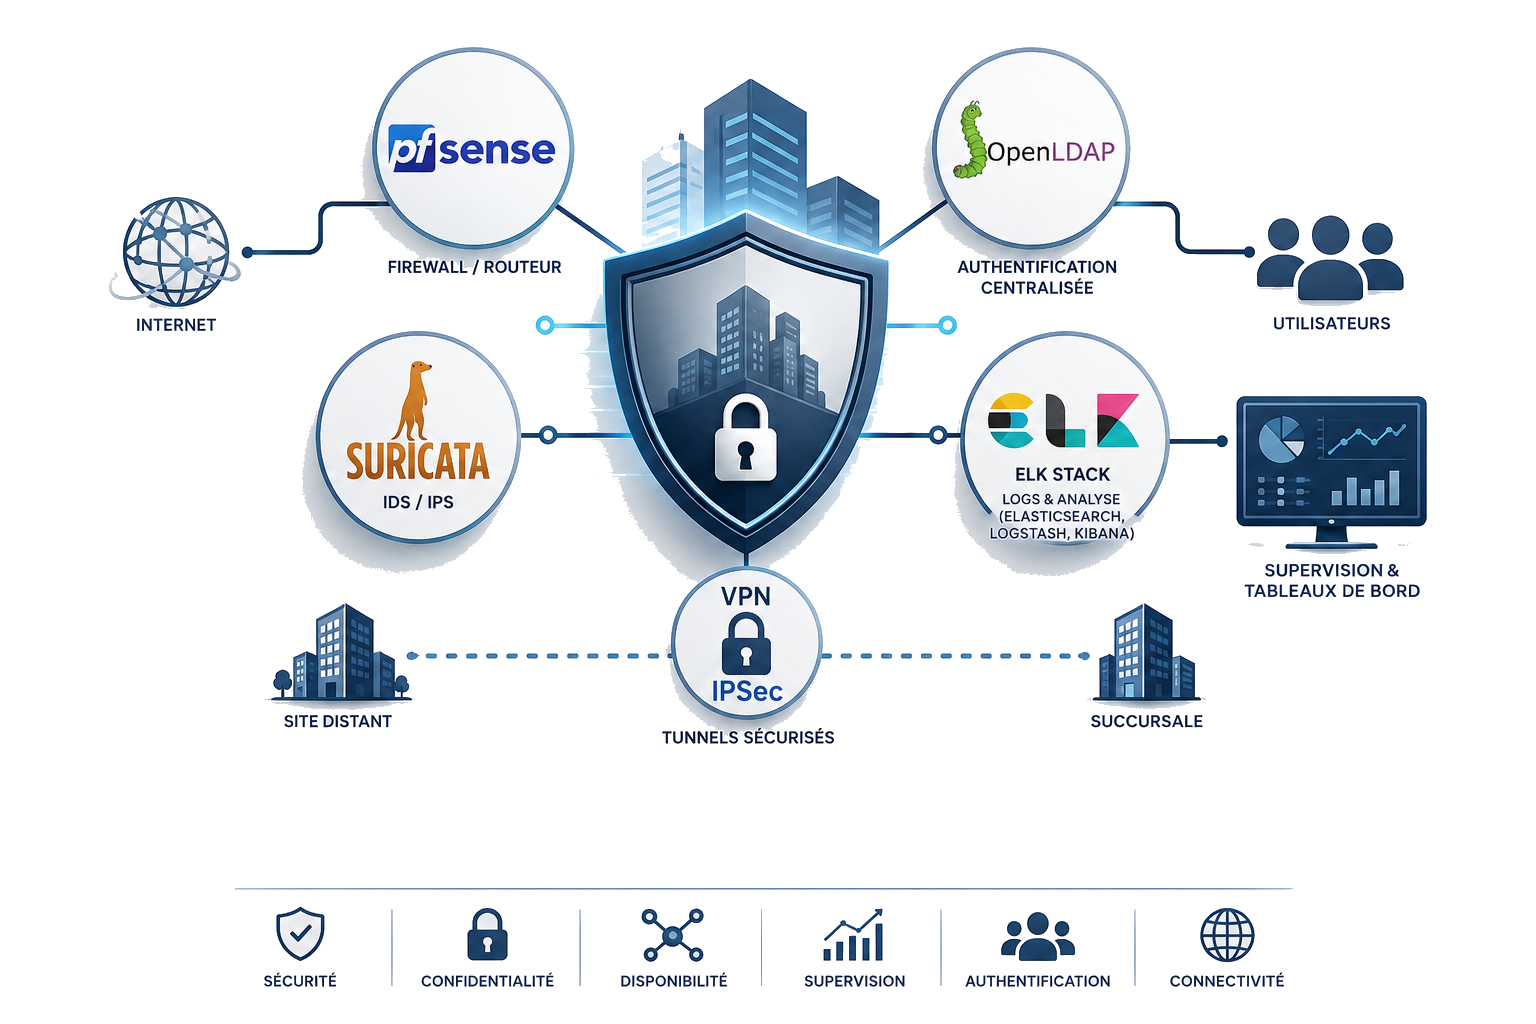
\includegraphics[width=0.75\linewidth,keepaspectratio]{screenshots/logo.png}}}

    \vspace{0.6cm}

    \textcolor{rulecolor}{\rule{0.52\linewidth}{0.45pt}}

    \vspace{0.7cm}

    \begin{minipage}[t]{0.40\linewidth}
      \raggedright
      \textcolor{graytext}{\footnotesize\scshape Realise par}\\[0.45em]
      {\large\bfseries\color{primary} El Gorrim Mohamed}\\[0.25em]
      {\large\bfseries\color{primary} Kchibal Ismail}\\[0.25em]
      {\large\bfseries\color{primary} Junaid Uthman}
    \end{minipage}%
    \hspace{0.12\linewidth}%
    \begin{minipage}[t]{0.40\linewidth}
      \raggedleft
      \textcolor{graytext}{\footnotesize\scshape Encadre par}\\[0.45em]
      {\large\bfseries\color{primary} Pr. Boudhir Anouar Abdelhakim}
    \end{minipage}

  \end{center}

  %-- Bandeau inférieur -------------------------------------------
  \vfill
  \noindent
  \begin{tcolorbox}[
    enhanced, sharp corners,
    colback=softbg, colframe=rulecolor,
    boxrule=0pt, toprule=0.45pt, arc=0pt,
    left=2.5cm, right=2.5cm,
    top=0.85cm, bottom=0.85cm,
    width=\paperwidth
  ]
    \centering
    \textcolor{graytext}{%
      \small Annee Universitaire\enspace
      \textbf{2025\,--\,2026}\enspace\textbullet\enspace\today}
  \end{tcolorbox}

  \restoregeometry
\end{titlepage}

%------------------------------------------------------------------
% Table des matières
%------------------------------------------------------------------
\setcounter{tocdepth}{2}
{\setlength{\parskip}{0pt}\tableofcontents}
\clearpage

% ═════════════════════════════════════════════════════════════════════
\section{Contexte et objectifs du projet}
% ═════════════════════════════════════════════════════════════════════

La societe MOBITECH, une PME d'une quatre-vingtaine d'employes repartis sur deux sites -- un siege principal et une agence distante -- ne disposait d'aucune infrastructure reseau structuree au demarrage de ce projet. Notre mission a ete de concevoir, deployer et securiser de bout en bout cette infrastructure, en partant de zero jusqu'a une architecture operationnelle et durcie.

L'ensemble du projet a ete realise dans GNS3 version 2.2, qui nous a permis d'executer des machines virtuelles QEMU (pfSense, Debian 12) et des conteneurs Docker dans un reseau entierement virtualise. Toutes les configurations documentees dans ce rapport ont ete effectivement appliquees et testees -- les captures d'ecran presentees sont issues de l'environnement de production simule.

\begin{tcolorbox}[colback=primarylight,colframe=primary!40,arc=4pt,boxrule=0.6pt,
  left=8pt,right=8pt,top=6pt,bottom=6pt,before skip=0.5em,after skip=0.5em]
\textbf{Perimetre technique :}
\begin{itemize}[nosep,leftmargin=1.2em]
  \item Pare-feu pfSense CE 2.8.1 (siege et agence) avec segmentation VLAN et DMZ
  \item Tunnel VPN IPSec IKEv2 site-a-site siege~$\leftrightarrow$~agence
  \item Deux serveurs Debian 12 (AD-LDAP, Fichiers) + trois conteneurs Docker (MariaDB, nginx, SMTP)
  \item Durcissement complet : SSH port 2222 + MFA TOTP, UFW, OpenLDAP, fail2ban, rkhunter, AIDE, sauvegardes GPG
  \item IDS Suricata 7.0 sur pfSense avec regles ETOpen (bonus)
  \item Stack ELK 8.13 pour la centralisation et la visualisation des journaux (bonus)
\end{itemize}
\end{tcolorbox}

% ═════════════════════════════════════════════════════════════════════
\section{Partie 1 -- Conception de la topologie reseau}
% ═════════════════════════════════════════════════════════════════════

\subsection{Schema de conception de l'architecture}

Avant toute implementation dans GNS3, nous avons concu un schema logique de l'infrastructure cible. Ce schema nous a servi de reference tout au long du projet pour verifier la coherence des flux et des zones de securite.

\fig{screenshots/architecture.png}{Schema de conception de l'architecture reseau -- etabli avant implementation dans GNS3}{fig:architecture-conception}

\subsection{Architecture generale}

Pour structurer notre infrastructure, nous avons opte pour un modele de securite en zones -- chaque zone etant isolee par pfSense et ne pouvant communiquer avec les autres que via des regles de filtrage explicites. Ce choix nous permet de limiter drastiquement la portee d'une compromission : si un poste employe est infecte, l'attaquant ne peut pas lateralement atteindre les serveurs internes ou la zone d'administration sans franchir plusieurs couches de filtrage.

\fig{screenshots/topology-gns3.png}{Topologie reseau complete dans GNS3}{fig:topo-gns3}

\fig{screenshots/topology-summary.png}{Vue d'ensemble de la topologie -- zones et flux}{fig:topo-summary}

Nous avons articule le reseau autour de quatre grandes zones, chacune avec un niveau de confiance distinct. L'idee etait que pfSense incarne la frontiere entre ces zones, appliquant des politiques differenciees selon la nature du trafic :

\begin{itemize}[leftmargin=1.4em]
  \item \textbf{WAN} : interface de sortie vers Internet, simulee par un noeud NAT GNS3 (192.168.122.0/24) representant le lien FAI. Un routeur \texttt{Routeur-FAI} est place entre le commutateur WAN et pfSense-Siege pour simuler le troncon operateur.
  \item \textbf{LAN} : reseau interne du siege, segmente en trois VLANs routes par pfSense (inter-VLAN routing via sous-interfaces dot1q).
  \item \textbf{DMZ} : zone demilitarisee, interface separee de pfSense, hebergeant les services accessibles depuis Internet.
  \item \textbf{Site Agence} : reseau distant connecte par VPN IPSec site-a-site, traite comme une extension de confiance limitee du reseau principal.
\end{itemize}

\subsection{Segmentation VLAN du LAN}

Plutot que de laisser tous les postes et serveurs sur un meme reseau plat, nous avons segmente le LAN interne en trois VLANs selon le principe du moindre privilege : chaque groupe d'hotes n'acces qu'aux ressources dont il a strictement besoin. Trois profils se sont naturellement degages -- les serveurs internes, les postes des employes, et le reseau d'administration -- auxquels nous avons associe un sous-reseau et des regles de filtrage distincts :

\begin{table}[H]
\centering
\begin{tabular}{@{}lllp{6cm}@{}}
\toprule
\textbf{VLAN} & \textbf{Nom} & \textbf{Sous-reseau} & \textbf{Hotes} \\
\midrule
10 & Serveurs internes & 192.168.10.0/24 & AD-LDAP (.10), Fichiers (.20), BDD-MariaDB (.30) \\
20 & Postes employes  & 192.168.20.0/24 & Employes 1--3 (DHCP : .100--.230) \\
30 & Administration   & 192.168.30.0/24 & Admin-PC (.10), Switch-Mgmt (.20), AP-WiFi (.30) \\
\bottomrule
\end{tabular}
\caption{Segmentation VLAN du reseau interne}
\label{tab:vlans}
\end{table}

Ce decoupage repond a deux objectifs complementaires. D'abord, contenir les incidents : un poste employe compromis (VLAN 20) ne peut pas atteindre directement les serveurs du VLAN 10, et encore moins le VLAN 30 d'administration. Ensuite, affiner les politiques : les serveurs ont des besoins reseau tres differents des postes utilisateurs, et les regles pfSense refletent exactement ces differences plutot que d'appliquer une politique uniforme trop permissive.

\subsection{Plan d'adressage IP complet}

\begin{longtable}{@{}lllll@{}}
\toprule
\textbf{Zone} & \textbf{Hote} & \textbf{Adresse IP} & \textbf{Masque} & \textbf{Passerelle} \\
\midrule
\endhead
WAN (simule) & pfSense-Siege vtnet0 & DHCP (192.168.122.x) & /24 & 192.168.122.1 \\
WAN (simule) & pfSense-Agence vtnet0 & DHCP (192.168.122.x) & /24 & 192.168.122.1 \\
\midrule
DMZ & pfSense-Siege (OPT1) & 192.168.50.1 & /24 & -- \\
DMZ & Web-Apache (nginx) & 192.168.50.10 & /24 & 192.168.50.1 \\
DMZ & Mail-Server (SMTP) & 192.168.50.20 & /24 & 192.168.50.1 \\
\midrule
VLAN 10 & pfSense-Siege (LAN.10) & 192.168.10.1 & /24 & -- \\
VLAN 10 & AD-LDAP & 192.168.10.10 & /24 & 192.168.10.1 \\
VLAN 10 & Fichiers & 192.168.10.20 & /24 & 192.168.10.1 \\
VLAN 10 & BDD-MariaDB & 192.168.10.30 & /24 & 192.168.10.1 \\
\midrule
VLAN 20 & pfSense-Siege (LAN.20) & 192.168.20.1 & /24 & -- \\
VLAN 20 & Employe-1 & DHCP (.100+) & /24 & 192.168.20.1 \\
VLAN 20 & Employe-2 & DHCP (.100+) & /24 & 192.168.20.1 \\
VLAN 20 & Employe-3 & DHCP (.100+) & /24 & 192.168.20.1 \\
\midrule
VLAN 30 & pfSense-Siege (LAN.30) & 192.168.30.1 & /24 & -- \\
VLAN 30 & Admin-PC & 192.168.30.10 & /24 & 192.168.30.1 \\
\midrule
Agence & pfSense-Agence (LAN) & 192.168.60.1 & /24 & -- \\
Agence & Agence-PC-1 & 192.168.60.10 & /24 & 192.168.60.1 \\
Agence & Agence-PC-2 & 192.168.60.20 & /24 & 192.168.60.1 \\
\bottomrule
\end{longtable}

\subsection{Justification des choix technologiques}

Nos choix technologiques ont ete guides par trois criteres : maturite en production, support natif des fonctionnalites requises, et facilite de gestion dans un contexte PME.

\textbf{pfSense CE 2.8.1} s'est impose comme pare-feu principal car il reunit en un seul outil tout ce dont nous avions besoin : gestion des VLANs 802.1Q, routage inter-VLAN, VPN IPSec IKEv2, serveur DHCP par interface, et une interface web complete -- le tout sans licence commerciale. La version 2.8.1, disponible via l'installateur reseau Netgate, est la plus recente a la date du projet et beneficie des correctifs de securite actifs.

\textbf{Debian 12 (Bookworm)} a ete retenu pour les serveurs Linux. Notre choix s'est porte sur cette distribution pour sa stabilite reconnue en production, son cycle de maintenance long, et le fait que systemd et AppArmor y sont actifs par defaut. Nous avons utilise le format cloud-init pour la configuration initiale (adresse IP statique, nom d'hote, compte root) afin de rendre le deploiement reproductible.

\textbf{Docker} (mariadb:latest, nginx:alpine, bytemark/smtp) a ete retenu pour les services BDD, Web et Mail : ces images officielles sont minimalistes et leur surface d'attaque est significativement reduite par rapport a une installation complete sur OS. Les images sont maintenues par leurs communautes respectives.

\textbf{GNS3} avec commutateurs Ethernet virtuels et ports dot1q nous a permis de simuler fidelement les VLANs 802.1Q sans materiel physique, tout en conservant la possibilite de transposer les configurations sur du materiel reel.

% ═════════════════════════════════════════════════════════════════════
\section{Partie 2 -- Securisation du reseau}
% ═════════════════════════════════════════════════════════════════════

\subsection{Installation de pfSense}

Notre premiere etape concrete a ete de deployer pfSense CE 2.8.1 sur deux machines virtuelles QEMU -- une pour le siege, une pour l'agence. L'installateur Netgate fonctionne en mode reseau : il telecharge les paquets directement depuis les serveurs Netgate, ce qui impliquait de verifier en amont que le noeud WAN (NAT GNS3) avait bien acces a Internet. Un detail qui peut bloquer si on ne l'anticipe pas.

\fig{screenshots/pfsense-installers-starting.png}{Demarrage de l'installateur Netgate pour pfSense-Siege et pfSense-Agence}{fig:pfsense-install}

\figw{screenshots/pfsense-version-selection.png}{Selection de la version 2.8.1}{fig:pfsense-version}{0.65}

Une fois l'installation terminee, nous avons utilise la console serie pour assigner les interfaces (vtnet0=WAN, vtnet1=LAN, vtnet2=OPT1/DMZ pour le siege) et definir l'adresse LAN initiale -- indispensable pour acceder ensuite a l'interface web de configuration.

\fig{screenshots/pfsense-console-menu.png}{Menu console pfSense apres demarrage (siege et agence)}{fig:pfsense-console}

\subsection{Configuration des interfaces et des VLANs}

Pour mettre en oeuvre la segmentation VLAN, nous avons cree les VLANs 10, 20 et 30 directement sur l'interface LAN (vtnet1) de pfSense-Siege. Chaque VLAN obtient sa propre sous-interface logique avec son adresse de passerelle -- c'est pfSense qui assure le routage inter-VLAN, eliminant le besoin d'un commutateur Layer 3 dedie.

\fig{screenshots/pfsense-vlans.png}{Creation des VLANs 10, 20 et 30 dans pfSense}{fig:pfsense-vlans}

\fig{screenshots/pfsense-vlan-interface-assignement.png}{Assignation des interfaces VLAN dans pfSense}{fig:pfsense-vlan-assign}

Cote commutation, le SW-LAN (noeud ethernet\_switch GNS3) a ete configure avec le port 0 en mode \texttt{dot1q} (lien trunk vers pfSense, transportant tous les VLANs tagues) et les ports 1, 2, 3 en mode acces vers les commutateurs d'acces SW-VLAN10, SW-VLAN20 et SW-VLAN30.

\subsection{DHCP pour le VLAN 20 (postes employes)}

Seul le VLAN 20 (postes employes) utilise le DHCP -- les serveurs et les equipements d'administration ont des adresses statiques pour des raisons de stabilite et de filtrage. Nous avons active le serveur DHCP integre de pfSense sur l'interface VLAN20, avec une plage de 192.168.20.100 a 192.168.20.230 et une duree de bail de 24h.

\figw{screenshots/pfsense-DHCP-vlan20.png}{Configuration DHCP pour le VLAN 20 dans pfSense}{fig:pfsense-dhcp}{0.75}

\subsection{Configuration du pare-feu}

\subsubsection{Politique par defaut}

Notre politique de filtrage repose sur le principe \emph{deny all} par defaut : pfSense bloque tout le trafic entrant sur chaque interface, et nous n'ouvrons que les flux dont le besoin est documente et justifie. Cette approche presente un avantage important -- si un service est malencontreusement ouvert sur un serveur, il reste inaccessible depuis le reseau tant qu'aucune regle pare-feu ne l'autorise explicitement.

\subsubsection{Regles WAN}

Sur l'interface WAN, notre choix a ete de bloquer l'integralite du trafic entrant initie depuis Internet. La seule exception concerne les paquets IKE/ESP du VPN IPSec, que pfSense gere automatiquement lors de la creation du tunnel. Tout autre trafic entrant non sollicite est bloque et journalise -- ce journal nous a d'ailleurs ete utile pour verifier que rien ne passait en dehors des flux attendus.

\fig{screenshots/pfsense-wan.rules.png}{Regles de filtrage sur l'interface WAN}{fig:pfsense-wan-rules}

\subsubsection{Regles inter-VLAN et DMZ}

Pour les flux inter-VLAN et vers la DMZ, nous avons adopte une approche minimaliste : n'autoriser que ce qui est strictement necessaire au fonctionnement metier, et bloquer tout le reste. Le tableau suivant recapitule les regles que nous avons definies :

\begin{table}[H]
\centering
\begin{tabular}{@{}lllll@{}}
\toprule
\textbf{Source} & \textbf{Destination} & \textbf{Port/Proto} & \textbf{Action} & \textbf{Motif} \\
\midrule
VLAN20 (employes) & VLAN10 (serveurs) & 389/tcp LDAP & ALLOW & Authentification \\
VLAN20 & VLAN10 & 445/tcp SMB & ALLOW & Partage fichiers \\
VLAN20 & DMZ & 80,443/tcp & ALLOW & Acces web interne \\
VLAN30 (admin) & Any & Any & ALLOW & Administration \\
VLAN10 & Any & Any & ALLOW & Serveurs internes \\
DMZ & Internet & 80,443/tcp & ALLOW & Sites web \\
Any & Any & Any & DENY & Politique par defaut \\
\bottomrule
\end{tabular}
\caption{Principales regles de filtrage inter-zones}
\label{tab:fw-rules}
\end{table}

\subsection{NAT sortant}

Pour que les hotes internes puissent atteindre Internet, nous avons configure le NAT sortant en mode \emph{Hybrid}. Ce mode nous convenait car pfSense genere automatiquement les regles NAT de base pour tous les sous-reseaux LAN/VLAN, tout en nous laissant la possibilite d'ajouter des regles manuelles si besoin -- une flexibilite utile sans complexite superflue.

\figw{screenshots/pfSense-NAT.png}{Configuration NAT sortant en mode Hybrid}{fig:pfsense-nat}{0.80}

\subsection{Securisation du routage et des acces d'administration}

pfSense jouant egalement le role de routeur inter-VLAN dans notre topologie, nous avons applique directement sur lui les bonnes pratiques de securisation habituellement recommandees pour les routeurs d'entreprise. L'idee etait de ne pas introduire de surface d'attaque supplementaire a travers l'equipement central du reseau :

\begin{itemize}[leftmargin=1.4em,noitemsep]
  \item \textbf{Pas de Telnet} : pfSense n'active pas Telnet. L'acces d'administration s'effectue exclusivement via HTTPS (interface web) ou SSH.
  \item \textbf{SSH restreint au VLAN30} : dans pfSense (\textit{System $\to$ Advanced $\to$ Secure Shell}), l'acces SSH est active uniquement depuis le sous-reseau 192.168.30.0/24 (VLAN Administration).
  \item \textbf{ACL par interface} : les regles de filtrage pfSense jouent le role des ACLs traditionnelles -- chaque interface n'autorise que les flux legitimes documentes dans le tableau~\ref{tab:fw-rules}. Tout le reste est bloque par la politique \emph{deny all} par defaut.
  \item \textbf{Pas de protocole de routage dynamique} : le reseau etant entierement sous pfSense (routage statique inter-VLAN), aucun protocole OSPF/RIP n'est necessaire. L'absence de protocole de routage dynamique elimine le risque d'injection de routes malveillantes.
  \item \textbf{Interface HTTP non chiffree desactivee} : seul HTTPS (port 443 interne) est accepte pour l'interface web pfSense. Le redirecteur HTTP est desactive.
\end{itemize}

\subsection{VPN IPSec site-a-site}

\subsubsection{Parametres IKE Phase 1}

\begin{table}[H]
\centering
\begin{tabular}{@{}ll@{}}
\toprule
\textbf{Parametre} & \textbf{Valeur} \\
\midrule
Version IKE & IKEv2 \\
Algorithme de chiffrement & AES-256-CBC \\
Algorithme de hachage & SHA-256 (HMAC\_SHA2\_256\_128) \\
Groupe DH & MODP-2048 (groupe 14) \\
Duree de vie Phase 1 & 28800 secondes (8h) \\
Mode d'authentification & Pre-shared key \\
Identifiant local/distant & Adresse IP WAN \\
\bottomrule
\end{tabular}
\caption{Parametres IKE Phase 1 du tunnel VPN}
\label{tab:ike-p1}
\end{table}

\subsubsection{Parametres IPSec Phase 2}

\begin{table}[H]
\centering
\begin{tabular}{@{}ll@{}}
\toprule
\textbf{Parametre} & \textbf{Valeur} \\
\midrule
Protocole & ESP \\
Chiffrement & AES-256-CBC \\
Hachage & SHA-256 \\
Groupe PFS & MODP-2048 \\
Duree de vie Phase 2 & 3600 secondes (1h) \\
Reseaux locaux & 192.168.10.0/24, 192.168.20.0/24, 192.168.30.0/24 \\
Reseaux distants & 192.168.60.0/24 \\
\bottomrule
\end{tabular}
\caption{Parametres IPSec Phase 2 du tunnel VPN}
\label{tab:ipsec-p2}
\end{table}

\fig{screenshots/pfsense-IPSec.png}{Configuration du tunnel IPSec sur pfSense-Siege}{fig:pfsense-ipsec}

\fig{screenshots/pfsense-IPSec-rules.png}{Regles de filtrage sur l'interface IPSec}{fig:pfsense-ipsec-rules}

\subsubsection{Etablissement du tunnel et verification}

Apres avoir reproduit la configuration symetrique sur pfSense-Agence (en inversant les reseaux locaux et distants), nous avons initie le tunnel. Le resultat a ete immediat : le statut IPSec affiche \texttt{Established} pour les deux phases, confirmant que la negotiation IKEv2 s'est deroulee correctement et que le canal chiffre est operationnel entre les deux sites.

\fig{screenshots/pfsense-connection-established.png}{Statut IPSec : tunnel etabli (Phase 1 et Phase 2 actives)}{fig:pfsense-vpn-ok}

\okbox{%
\textbf{Verification du tunnel :} Le statut affiche \texttt{Established} avec les algorithmes negoties :
\texttt{AES\_CBC(256)}, \texttt{HMAC\_SHA2\_256\_128}, \texttt{MODP\_2048}. La connectivite a ete
verifiee par ping depuis Admin-PC (192.168.30.10) vers Agence-PC-1 (192.168.60.10) a travers le tunnel chiffre.
}

\subsection{IDS Suricata sur pfSense}

Pour la detection d'intrusions, nous avons choisi de deployer Suricata 7.0.11 directement sur pfSense-Siege, en mode IDS passif -- c'est-a-dire en observation uniquement, sans blocage actif. Ce choix delibere s'explique par le contexte : en mode IPS inline, Suricata peut generer des faux positifs qui interrompent du trafic legitime ; en mode passif, nous disposons d'une visibilite complete sur les menaces sans risque d'impact sur la disponibilite. L'installation passe par le gestionnaire de paquets integre de pfSense, ce qui simplifie considerablement l'integration.

\begin{figure}[H]
  \centering
  {\setlength{\fboxsep}{3pt}\setlength{\fboxrule}{0.4pt}
  \fbox{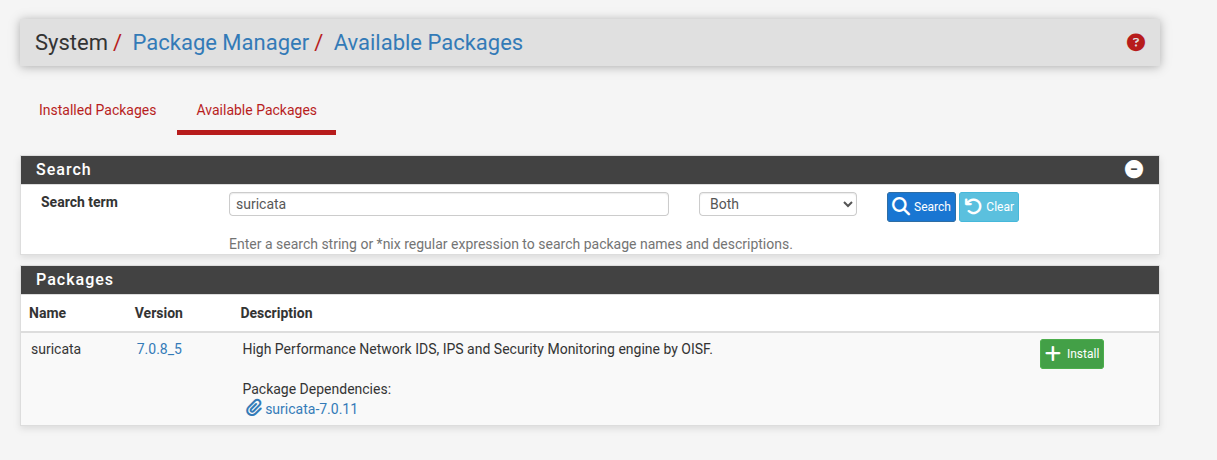
\includegraphics[width=0.90\linewidth,keepaspectratio]{screenshots/pfsense-suricata-available.png}}}
  \caption{Suricata disponible dans le gestionnaire de paquets pfSense}\label{fig:suricata-available}
\end{figure}

\begin{figure}[H]
  \centering
  {\setlength{\fboxsep}{3pt}\setlength{\fboxrule}{0.4pt}
  \fbox{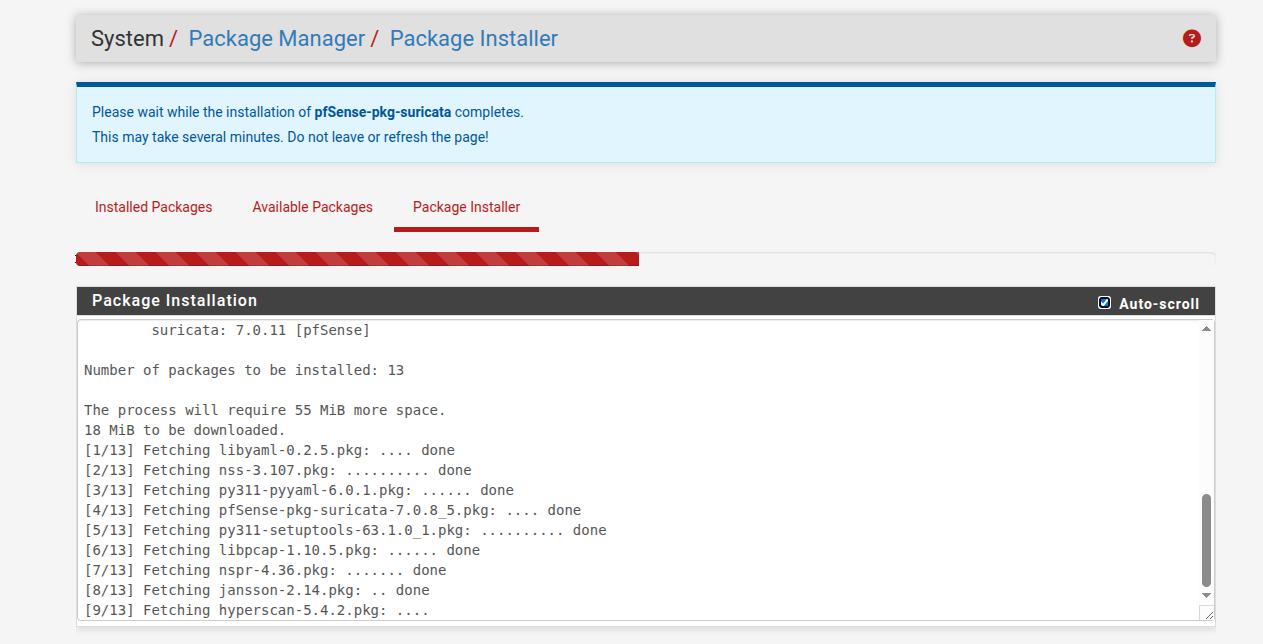
\includegraphics[width=0.90\linewidth,keepaspectratio]{screenshots/pfsense-suricata-installing.png}}}
  \caption{Installation de pfSense-pkg-suricata (13 paquets, 55 MiB)}\label{fig:suricata-installing}
\end{figure}

Nous avons configure deux instances Suricata en parallele -- une sur LAN (vtnet1) pour surveiller le trafic interne, et une sur WAN (vtnet0) pour capturer les tentatives d'acces depuis l'exterieur. Cette double instrumentation nous donne une couverture complete, aussi bien pour les menaces exterieures que pour les comportements anormaux internes :

\begin{itemize}[noitemsep]
  \item \textbf{Mode} : IDS passif (Block Offenders desactive)
  \item \textbf{Regles} : ETOpen Emerging Threats (mise a jour automatique)
  \item \textbf{Alertes} : envoyees vers le syslog systeme et en format EVE JSON
  \item \textbf{Pattern matching} : AUTO (Hyperscan active)
\end{itemize}

\begin{figure}[H]
  \centering
  {\setlength{\fboxsep}{3pt}\setlength{\fboxrule}{0.4pt}
  \fbox{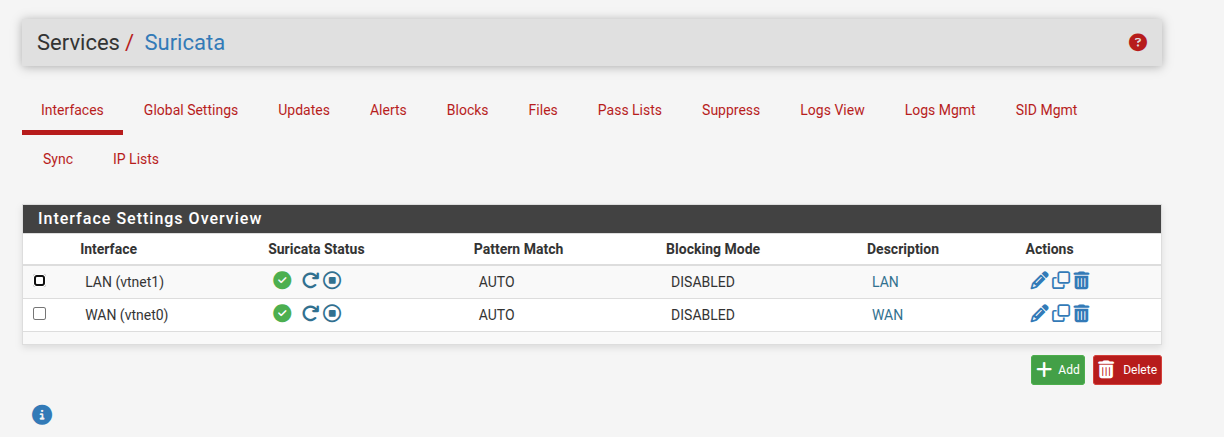
\includegraphics[width=0.90\linewidth,keepaspectratio]{screenshots/pfsense-suricata-started.png}}}
  \caption{Suricata actif sur LAN et WAN -- statut vert, mode IDS}\label{fig:suricata-started}
\end{figure}

Pour les signatures, nous avons opte pour les regles ETOpen (Emerging Threats Open), un ensemble communautaire mis a jour automatiquement et couvrant les principales familles de menaces actuelles. Les categories que nous avons activees sont directement pertinentes pour notre profil de risque :

\begin{itemize}[noitemsep,leftmargin=1.4em]
  \item \textbf{scan} : detection des scans de ports Nmap (SYN scan, NULL scan, XMAS scan)
  \item \textbf{emerging-dos} : detection des tentatives de brute-force et flooding
  \item \textbf{emerging-exploit} : detection des tentatives d'exploitation connues
  \item \textbf{emerging-malware} : signatures de trafic malveillant et C2
\end{itemize}

\begin{figure}[H]
  \centering
  {\setlength{\fboxsep}{3pt}\setlength{\fboxrule}{0.4pt}
  \fbox{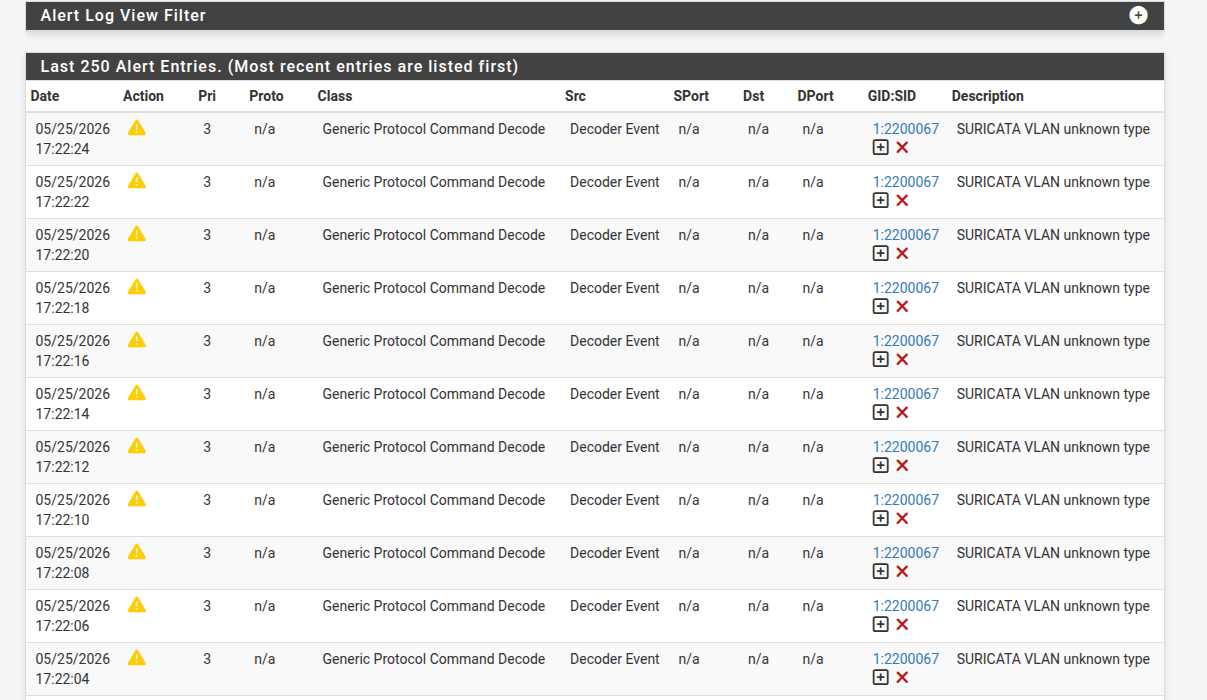
\includegraphics[width=0.90\linewidth,keepaspectratio]{real-results/alerts-tab.png}}}
  \caption{Onglet Alerts de Suricata dans pfSense -- alertes reelles capturees en temps reel}\label{fig:suricata-alerts-tab}
\end{figure}

Les alertes generees par Suricata (dont des alertes \texttt{SURICATA VLAN unknown type} et des evenements IKE du tunnel VPN) sont visibles en temps reel dans la stack ELK documentee en section~\ref{sec:elk}.

% ═════════════════════════════════════════════════════════════════════
\section{Partie 3 -- Securisation des serveurs Linux}
% ═════════════════════════════════════════════════════════════════════

Une fois le reseau en place, nous nous sommes attaques a la securisation des serveurs eux-memes. Notre philosophie pour cette partie etait de partir de la surface d'attaque minimale : desactiver tout ce qui n'est pas necessaire, n'ouvrir que ce qui l'est, et controler chaque point d'entree. Le durcissement a ete applique aux deux serveurs Debian 12 (AD-LDAP et Fichiers). Pour garantir la reproductibilite et eviter les oublis, nous avons developpe un script shell \texttt{harden\_server.sh} qui automatise l'ensemble des operations -- il est documente en section~\ref{sec:script}.

\subsection{Mise a jour et services inutiles}

Notre premier geste sur chaque serveur a ete de l'amener a un etat de base propre avant d'y toucher : mise a jour complete des paquets, activation des mises a jour de securite automatiques, et desactivation des services inutiles. Cette etape est fondamentale -- inutile de construire une configuration de securite sur un systeme qui porte deja des vulnerabilites corrigees depuis des mois.

\begin{lstlisting}[caption={Mise a jour et desactivation des services inutiles}]
apt-get update -q && apt-get upgrade -y -q
apt-get install -y unattended-upgrades apt-listchanges
dpkg-reconfigure -f noninteractive unattended-upgrades

for svc in cups avahi-daemon bluetooth ModemManager; do
    systemctl stop $svc 2>/dev/null || true
    systemctl disable $svc 2>/dev/null || true
done

timedatectl set-timezone Africa/Casablanca
apt-get install -y chrony
systemctl enable chrony && systemctl start chrony
\end{lstlisting}

Le paquet \texttt{unattended-upgrades} est configure pour appliquer automatiquement les mises a jour de securite Debian sans intervention manuelle.

\subsection{Securisation SSH}

La securisation de SSH a ete notre priorite numero un -- c'est le principal vecteur d'acces administratif, et par consequent la cible de choix pour un attaquant. Nous avons reconfigure le daemon SSH pour ne repondre qu'aux connexions satisfaisant des criteres stricts :

\begin{lstlisting}[caption={Extrait de /etc/ssh/sshd\_config applique}]
Port 2222
Protocol 2
PermitRootLogin no
MaxAuthTries 3
MaxSessions 5
PubkeyAuthentication yes
PasswordAuthentication no
PermitEmptyPasswords no
ChallengeResponseAuthentication yes
AuthenticationMethods publickey,keyboard-interactive
AllowUsers adminit
LoginGraceTime 30
ClientAliveInterval 300
ClientAliveCountMax 2
X11Forwarding no
Banner /etc/ssh/banner
SyslogFacility AUTH
LogLevel VERBOSE
\end{lstlisting}

Quelques points meritent une explication sur le raisonnement qui nous a conduits a ces choix :
\begin{itemize}[leftmargin=1.4em]
  \item \textbf{Port 2222} : deplace du port standard 22 pour reduire le bruit dans les logs (scanners automatiques).
  \item \textbf{PermitRootLogin no} : l'acces direct en root via SSH est impossible. L'administration se fait via un compte \texttt{adminit} avec elevation \texttt{sudo}.
  \item \textbf{PasswordAuthentication no + AuthenticationMethods publickey,keyboard-interactive} : l'authentification requiert a la fois une cle publique RSA 4096 et un code TOTP (Google Authenticator), realisant le MFA.
  \item \textbf{AllowUsers adminit} : liste blanche explicite, tout autre compte systeme ne peut pas ouvrir de session SSH meme s'il possede un mot de passe valide.
  \item \textbf{ClientAliveInterval 300 / CountMax 2} : une session inactive depuis plus de 10 minutes est automatiquement fermee.
\end{itemize}

\subsection{Pare-feu local UFW}

Le pare-feu pfSense filtre le trafic au niveau reseau, mais cela ne suffit pas : un attaquant qui aurait acces a un VLAN autorise pourrait tout de meme atteindre des ports non voulus sur un serveur. Nous avons donc ajoute une deuxieme couche de defense avec UFW (pare-feu local sur chaque serveur), selon une philosophie de defense en profondeur. La politique d'entree est \emph{deny all} par defaut, et nous n'ouvrons que les ports strictement necessaires, avec restriction supplementaire par sous-reseau source :

\begin{lstlisting}[caption={Regles UFW appliquees sur le serveur AD-LDAP}]
ufw default deny incoming
ufw default allow outgoing

# SSH uniquement depuis le VLAN d'administration
ufw allow from 192.168.30.0/24 to any port 2222 proto tcp

# LDAP/LDAPS uniquement depuis le reseau interne
ufw allow from 192.168.10.0/24 to any port 389 proto tcp
ufw allow from 192.168.10.0/24 to any port 636 proto tcp

# MariaDB depuis VLAN10 et VLAN20 seulement
ufw allow from 192.168.10.0/24 to any port 3306 proto tcp
ufw allow from 192.168.20.0/24 to any port 3306 proto tcp

ufw --force enable
\end{lstlisting}

Verification en production sur AD-LDAP (\texttt{ufw status verbose}) :

\begin{lstlisting}[caption={Sortie reelle -- ufw status verbose sur AD-LDAP (192.168.10.10)}]
Status: active
Logging: on (low)
Default: deny (incoming), allow (outgoing), disabled (routed)

To                         Action      From
--                         ------      ----
2222/tcp       ALLOW IN    192.168.30.0/24   # SSH Admin VLAN30
80/tcp         ALLOW IN    Anywhere          # HTTP
443/tcp        ALLOW IN    Anywhere          # HTTPS
389/tcp        ALLOW IN    192.168.10.0/24   # LDAP internal
636/tcp        ALLOW IN    192.168.10.0/24   # LDAPS
3306/tcp       ALLOW IN    192.168.10.0/24   # MariaDB VLAN10
3306/tcp       ALLOW IN    192.168.20.0/24   # MariaDB VLAN20
\end{lstlisting}

Sur le serveur Fichiers (192.168.10.20), les regles UFW adaptees au role de partage de fichiers :

\begin{lstlisting}[caption={Sortie reelle -- ufw status verbose sur Fichiers (192.168.10.20)}]
Status: active
Default: deny (incoming), allow (outgoing)

To                         Action      From
--                         ------      ----
2222/tcp       ALLOW IN    192.168.30.0/24   # SSH Admin VLAN30
445/tcp        ALLOW IN    192.168.10.0/24   # Samba VLAN10
445/tcp        ALLOW IN    192.168.20.0/24   # Samba VLAN20
139/tcp        ALLOW IN    192.168.10.0/24   # NetBIOS VLAN10
139/tcp        ALLOW IN    192.168.20.0/24   # NetBIOS VLAN20
2049/tcp       ALLOW IN    192.168.10.0/24   # NFS VLAN10
2049/tcp       ALLOW IN    192.168.20.0/24   # NFS VLAN20
\end{lstlisting}

La politique \texttt{deny incoming} par defaut bloque egalement les requetes ICMP non sollicitees (ping flood, Smurf). Aucune regle UFW n'ouvre le protocole ICMP, ce qui constitue une protection anti-flood implicite.

\subsection{Durcissement Apache et HTTPS}

Sur le serveur Web-Apache (DMZ), Apache 2.4 a ete configure pour masquer les informations de version et forcer le HTTPS :

\begin{lstlisting}[caption={Directives de securite Apache -- /etc/apache2/conf-enabled/security.conf}]
ServerTokens Prod
ServerSignature Off
TraceEnable Off
Header always set X-Content-Type-Options nosniff
Header always set X-Frame-Options DENY
Header always set X-XSS-Protection "1; mode=block"
\end{lstlisting}

Un certificat auto-signe RSA 2048 bits a ete genere pour mobitech.local. Le VirtualHost HTTP redirige systematiquement vers HTTPS. Les protocoles SSLv2, SSLv3, TLSv1 et TLSv1.1 sont desactives ; seuls TLS 1.2 et TLS 1.3 sont acceptes.

Pour le conteneur nginx (WEB1 Docker), des en-tetes de securite equivalents ont ete ajoutes a la configuration \texttt{/etc/nginx/conf.d/default.conf} et \texttt{server\_tokens off} a ete active.

\subsection{Securisation MariaDB}

MariaDB a ete securise en suivant les etapes equivalentes a \texttt{mysql\_secure\_installation} :

\begin{lstlisting}[caption={Securisation du compte root et suppression des donnees de test}]
DELETE FROM mysql.user WHERE User='';
DELETE FROM mysql.user WHERE User='root'
    AND Host NOT IN ('localhost','127.0.0.1','::1');
DROP DATABASE IF EXISTS test;
DELETE FROM mysql.db WHERE Db='test' OR Db='test\_%';
ALTER USER 'root'@'localhost' IDENTIFIED BY 'Mobitech2024!';
FLUSH PRIVILEGES;
\end{lstlisting}

\infobox{%
\textbf{Note technique -- Authentification unix\_socket :} Sur Debian 12, MariaDB installe par defaut le compte root avec le plugin \texttt{mysql\_native\_password}, contrairement a ce qu'indique la documentation officielle. L'acces via \texttt{mariadb -u root} echoue avec erreur 1045. La resolution a consiste a demarrer MariadB avec \texttt{--skip-grant-tables}, migrer root vers le plugin \texttt{unix\_socket}, puis relancer le service normalement.
}

L'adresse d'ecoute (\texttt{bind-address}) est restreinte a l'IP interne du serveur concerne. Verification en production :

\begin{lstlisting}[caption={Sortie reelle -- comptes MariaDB sur AD-LDAP apres securisation}]
MariaDB> SELECT user, host, plugin FROM mysql.user;
+-------------+-----------+-----------------------+
| User        | Host      | plugin                |
+-------------+-----------+-----------------------+
| mariadb.sys | localhost | mysql_native_password |
| root        | localhost | mysql_native_password |
| mysql       | localhost | mysql_native_password |
+-------------+-----------+-----------------------+
-- root@% supprime, base test supprimee, acces reseau bloque
\end{lstlisting}

\subsubsection{Note sur le service FTP}

L'architecture retenue n'integre pas de serveur FTP. Le partage de fichiers internes est assure par Samba (SMB/445) sur le serveur Fichiers, accessible uniquement depuis VLAN10 et VLAN20. Ce choix reduit la surface d'attaque : FTP transmet les identifiants en clair (meme en mode FTPS, la negotiation initiale est sensible) et Samba avec authentification NTLM/Kerberos est plus adapte a un environnement avec annuaire LDAP. L'absence de FTP eliminse le besoin de configurer vsftpd, chroot jail et les regles UFW associees.

% ═════════════════════════════════════════════════════════════════════
\section{Partie 4 -- Gestion des identites et des acces (IAM)}
% ═════════════════════════════════════════════════════════════════════

La gestion des identites est le fil conducteur de toute la securite : si n'importe qui peut se connecter avec n'importe quel compte, les controles reseau ne servent pas a grand chose. Notre approche IAM s'articule autour d'un annuaire centralise OpenLDAP, d'une politique de mots de passe stricte, et d'un MFA sur SSH -- trois couches qui se renforcent mutuellement.

\subsection{Annuaire OpenLDAP}

Pour centraliser la gestion des identites, nous avons opte pour OpenLDAP (slapd 2.5.13) sur le serveur AD-LDAP. Notre choix d'OpenLDAP repose sur plusieurs considerations : c'est une solution eprouvee, parfaitement integree dans les ecosystemes Linux, qui nous permet de gerer les comptes utilisateurs de facon centralisee sans dependre d'une solution proprietaire. Le domaine configure est \texttt{mobitech.local} (base DN : \texttt{dc=mobitech,dc=local}), avec une structure refletant l'organisation de la PME.

\subsubsection{Structure organisationnelle}

Nous avons structure l'annuaire en quatre unites organisationnelles (OUs) correspondant aux departements de la PME. Cette organisation facilite la delegation administrative et l'application de politiques differenciees par equipe :

\begin{lstlisting}[caption={Creation des OUs dans l'annuaire LDAP}]
ldapadd -x -D "cn=admin,dc=mobitech,dc=local" -w "Mobitech2024!" \
        -f /tmp/mobitech_ou.ldif

# Contenu du fichier LDIF :
# ou=Direction,dc=mobitech,dc=local
# ou=RH,dc=mobitech,dc=local
# ou=IT,dc=mobitech,dc=local
# ou=Commercial,dc=mobitech,dc=local
\end{lstlisting}

\begin{table}[H]
\centering
\begin{tabular}{@{}llll@{}}
\toprule
\textbf{OU} & \textbf{DN complet} & \textbf{Utilisateurs crees} & \textbf{UID Number} \\
\midrule
IT & ou=IT,dc=mobitech,dc=local & adminit & 2000 \\
Direction & ou=Direction,dc=mobitech,dc=local & directeur & 2001 \\
RH & ou=RH,dc=mobitech,dc=local & -- & -- \\
Commercial & ou=Commercial,dc=mobitech,dc=local & -- & -- \\
\bottomrule
\end{tabular}
\caption{Structure de l'annuaire LDAP de l'entreprise}
\label{tab:ldap-ous}
\end{table}

Les comptes utilisateurs sont de type \texttt{inetOrgPerson} + \texttt{posixAccount}, ce qui permet leur utilisation a la fois pour l'authentification LDAP et pour la resolution d'identite POSIX sur les serveurs Linux (via SSSD). Le schema POSIX (uidNumber, gidNumber, homeDirectory) est configure en prevision de l'integration SSSD.

\begin{tcolorbox}[colback=softbg,colframe=codeframe,arc=4pt,boxrule=0.5pt,
  left=8pt,right=8pt,top=6pt,bottom=6pt,before skip=0.5em,after skip=0.5em]
\textbf{Integration SSSD (en cours) :} L'installation de \texttt{sssd} + \texttt{libnss-ldap} sur les postes VLAN20 permettrait l'authentification systeme centralisee via LDAP. Le schema \texttt{posixAccount} est deja en place. Cette etape necessite des postes Linux Debian/Ubuntu dans VLAN20 (actuellement des noeuds VPCS dans GNS3, sans OS Linux complet).
\end{tcolorbox}

\subsubsection{Reinitialisation du mot de passe administrateur LDAP}

La commande \texttt{dpkg-reconfigure -f noninteractive slapd} n'applique pas toujours les \\ \texttt{debconf-set-selections} preconfigurees. Le mot de passe administrateur LDAP a ete redefini via l'API interne SASL/EXTERNAL (acces direct par socket unix, sans mot de passe) :

\begin{lstlisting}[caption={Reset du mot de passe admin LDAP via SASL/EXTERNAL}]
NEW_HASH=$(slappasswd -s "Mobitech2024!")
ldapmodify -Y EXTERNAL -H ldapi:/// << EOF
dn: olcDatabase={1}mdb,cn=config
changetype: modify
replace: olcRootPW
olcRootPW: $NEW_HASH
EOF
\end{lstlisting}

\subsection{Politique de mots de passe}

Le module PAM \texttt{pam\_pwquality} est configure pour imposer les contraintes suivantes :

\begin{lstlisting}[caption={/etc/security/pwquality.conf}]
minlen = 12       # longueur minimale 12 caracteres
dcredit = -1      # au moins 1 chiffre obligatoire
ucredit = -1      # au moins 1 majuscule obligatoire
lcredit = -1      # au moins 1 minuscule obligatoire
ocredit = -1      # au moins 1 caractere special obligatoire
remember = 12     # interdire la reutilisation des 12 derniers mots de passe
maxrepeat = 3     # pas plus de 3 caracteres identiques consecutifs
\end{lstlisting}

Le changement de mot de passe est force a la premiere connexion pour tout nouveau compte via :

\begin{lstlisting}[caption={Forcer le changement de MDP a la premiere connexion}]
chage -d 0 <username>   # expiration immediate -- MDP doit etre change
\end{lstlisting}

\subsection{Authentification multi-facteurs (MFA) pour SSH}

Google Authenticator (TOTP, RFC 6238) a ete installe via \texttt{libpam-google-authenticator}. La configuration PAM pour SSH combine la cle publique et le TOTP :

\begin{lstlisting}[caption={/etc/pam.d/sshd -- MFA SSH (configuration reelle)}]
auth required pam_google_authenticator.so nullok debug
@include common-account
@include common-session
@include common-password
session required pam_limits.so
\end{lstlisting}

\textbf{Note technique :} L'ajout de \texttt{UsePAM yes} dans \texttt{sshd\_config} est indispensable -- sans cette directive, le module \texttt{keyboard-interactive} de sshd ne fait pas appel a PAM et aucun prompt TOTP n'est envoye au client (echec silencieux). La directive \texttt{pam\_unix.so try\_first\_pass} a ete retiree car elle tentait d'utiliser le code TOTP comme mot de passe Unix, provoquant un echec immediat.

Combinee avec \texttt{AuthenticationMethods publickey,keyboard-interactive} dans \texttt{sshd\_config}, cette configuration impose : \textbf{cle ED25519} + \textbf{code TOTP a 6 chiffres}. La sequence d'authentification reelle est la suivante :

\begin{enumerate}[leftmargin=1.4em]
  \item Le client presente sa cle publique (verifiee contre \texttt{authorized\_keys}).
  \item sshd declenche le challenge \texttt{keyboard-interactive} via PAM.
  \item L'invite \texttt{Verification code:} apparait -- l'utilisateur saisit le code TOTP depuis Google Authenticator.
  \item Si les deux facteurs sont valides, la session s'ouvre avec affichage du banner MOBITECH.
\end{enumerate}

\begin{figure}[H]
  \centering
  {\setlength{\fboxsep}{3pt}\setlength{\fboxrule}{0.4pt}
  \fbox{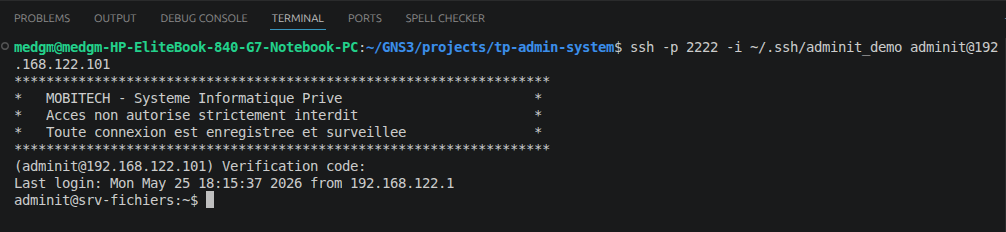
\includegraphics[width=0.90\linewidth,keepaspectratio]{real-results/ssh-login.png}}}
  \caption{Connexion SSH reelle -- banner MOBITECH + invite TOTP + session ouverte}\label{fig:ssh-mfa-login}
\end{figure}

\begin{figure}[H]
  \centering
  {\setlength{\fboxsep}{3pt}\setlength{\fboxrule}{0.4pt}
  \fbox{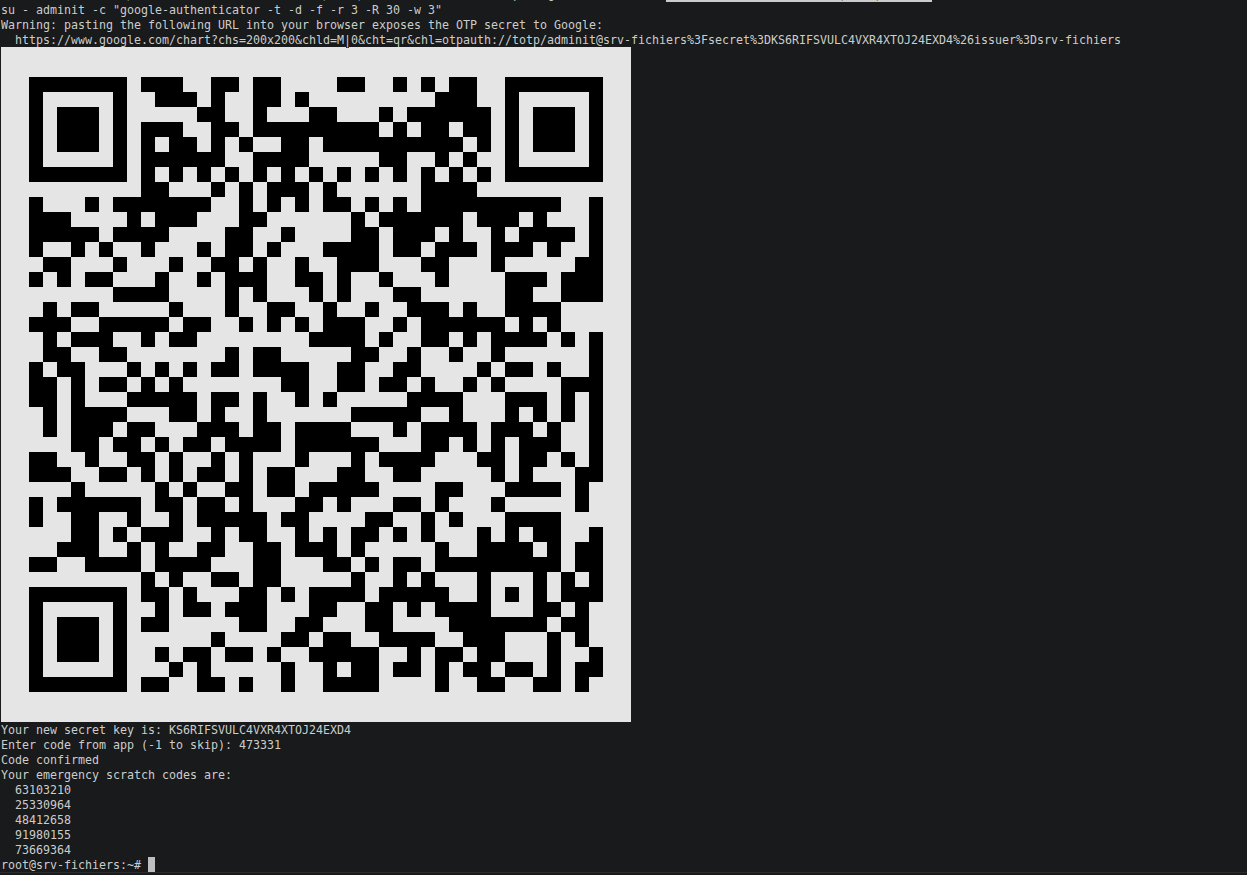
\includegraphics[width=0.90\linewidth,keepaspectratio]{real-results/google auth.png}}}
  \caption{Application Google Authenticator -- token TOTP 30s pour adminit@srv-fichiers}\label{fig:google-auth-app}
\end{figure}

L'option \texttt{nullok} permet aux comptes n'ayant pas encore configure leur token TOTP de se connecter avec la cle seule -- utile lors de la phase de provisionnement.

\subsection{Gestion granulaire des privileges (sudo)}

Les droits sudo sont definis par groupe dans \texttt{/etc/sudoers.d/mobitech} :

\begin{lstlisting}[caption={/etc/sudoers.d/mobitech}]
# Groupe IT : sudo complet
%it ALL=(ALL:ALL) ALL

# Operateurs : redemarrage et statut des services seulement
%operators ALL=(ALL) NOPASSWD: /bin/systemctl restart *, \
                               /bin/systemctl status *

# Journalisation complete de toutes les commandes sudo
Defaults logfile=/var/log/sudo.log
Defaults log_input, log_output
\end{lstlisting}

Les comptes systeme non utilises (\texttt{games}, \texttt{news}, \texttt{uucp}, \texttt{proxy}, \texttt{list}, \texttt{irc}, \texttt{gnats}) ont ete supprimes avec \texttt{userdel}. La limite de connexions simultanees par utilisateur est fixee a 3 via \texttt{/etc/security/limits.conf}.

% ═════════════════════════════════════════════════════════════════════
\section{Partie 5 -- Surveillance, journalisation et reponse aux incidents}
% ═════════════════════════════════════════════════════════════════════

Un reseau bien configure mais non surveille reste aveugle : on ne sait pas ce qui s'y passe, et surtout on ne detecte pas les incidents a temps. Notre approche de surveillance repose sur trois niveaux complementaires -- centralisation des journaux, reponse automatique aux attaques, et detection de modifications systeme -- pour s'assurer qu'une anomalie ne passe pas inapercue.

\subsection{Centralisation des journaux avec rsyslog}

L'idee centrale est simple : si un serveur est compromis, l'attaquant peut effacer ses propres traces localement. En centralisant les journaux sur un serveur tiers des leur emission, on s'assure que ces traces sont deja hors de portee au moment de la compromission. Nous avons donc configure rsyslog sur chaque serveur pour transferer tous les journaux vers AD-LDAP (192.168.10.10) sur le port 514 UDP :

\begin{lstlisting}[caption={Ajout dans /etc/rsyslog.conf sur chaque serveur}]
# Envoi centralise vers AD-LDAP
*.* @192.168.10.10:514

# Permissions sur les fichiers de logs locaux
$FileOwner root
$FileGroup adm
$FileCreateMode 0640
$DirCreateMode 0755
\end{lstlisting}

AD-LDAP devient ainsi le point de collecte central de l'infrastructure. Les journaux y arrivent en temps reel : en cas de compromission d'un serveur applicatif, les traces sont deja transmises et l'attaquant ne peut pas les effacer.

Nous avons verifie en production que les quatre services critiques d'AD-LDAP sont bien actifs apres durcissement :

\begin{lstlisting}[caption={Sortie reelle -- etat des services sur AD-LDAP}]
$ systemctl is-active ssh fail2ban mariadb slapd
active    <- sshd en ecoute sur port 2222
active    <- fail2ban surveille 3 jails (sshd, apache-auth, apache-badbots)
active    <- MariaDB bind sur 192.168.10.10
active    <- OpenLDAP slapd dc=mobitech,dc=local
\end{lstlisting}

\begin{lstlisting}[caption={Sortie reelle -- fail2ban jails actives}]
$ fail2ban-client status
Status
|- Number of jail:  3
`- Jail list:       apache-auth, apache-badbots, sshd
\end{lstlisting}

\subsection{Detection de brute-force avec fail2ban}

Plutot que de surveiller manuellement les logs et de bloquer les attaquants a la main, nous avons mis en place fail2ban pour automatiser cette reponse. Le principe est direct : fail2ban lit les journaux d'authentification en continu et, des qu'une source depasse un seuil de tentatives echouees, il l'inscrit dans iptables/nftables pour la duree configuree. Notre configuration cible les vecteurs d'attaque les plus frequents :

\begin{lstlisting}[caption={/etc/fail2ban/jail.local}]
[DEFAULT]
bantime  = 86400   # bannissement 24 heures
findtime = 600     # fenetre d'observation 10 minutes
maxretry = 5       # 5 tentatives max avant bannissement
backend  = systemd
destemail = admin@mobitech.local
action = %(action_mwl)s  # ban + mail + whois + log

[sshd]
enabled  = true
port     = 2222
logpath  = %(sshd_log)s
maxretry = 5

[apache-auth]
enabled  = true
port     = http,https
logpath  = %(apache_error_log)s

[apache-badbots]
enabled  = true
port     = http,https
logpath  = %(apache_access_log)s
maxretry = 2
\end{lstlisting}

Sur le serveur Mail-Server, nous avons complete cette configuration avec des jails supplementaires couvrant Postfix et Dovecot, ciblant les tentatives de force brute sur les protocoles mail.

\subsection{Verification d'integrite et detection de rootkits}

\subsubsection{rkhunter}

rkhunter (Rootkit Hunter) scanne le systeme a la recherche de rootkits connus, fichiers suspects, et modifications de permissions. La base de references a ete construite apres l'installation :

\begin{lstlisting}[caption={Initialisation de rkhunter}]
rkhunter --update --quiet     # mise a jour de la base de signatures
rkhunter --propupd --quiet    # enregistrement des proprietes actuelles
\end{lstlisting}

\subsubsection{AIDE}

AIDE (Advanced Intrusion Detection Environment) maintient une base de donnees cryptographique des fichiers du systeme. Toute modification (permissions, contenu, proprietaire) est detectee lors du prochain scan :

\begin{lstlisting}[caption={Initialisation de la base AIDE}]
aideinit                                           # creation de la base initiale
cp /var/lib/aide/aide.db.new /var/lib/aide/aide.db # activation
\end{lstlisting}

Verification en production -- base AIDE initialisee et rkhunter operationnel :

\begin{lstlisting}[caption={Sortie reelle -- verification rkhunter et aide sur AD-LDAP}]
$ rkhunter --version
Rootkit Hunter 1.4.6

$ ls -lh /var/lib/aide/aide.db
-rw------- 1 root root 10M May 25 03:06 /var/lib/aide/aide.db
# Base AIDE de 10 Mo initialisee le 25 mai 2026 a 03:06
# Contient les empreintes SHA512 de tous les fichiers systeme
\end{lstlisting}

Un scan hebdomadaire est programme via cron :

\begin{lstlisting}[caption={/etc/cron.weekly/security-scan}]
#!/bin/bash
rkhunter --check --skip-keypress --report-warnings-only \
    | mail -s "rkhunter $(hostname)" admin@mobitech.local
aide --check \
    | mail -s "aide integrity $(hostname)" admin@mobitech.local
\end{lstlisting}

\subsection{Sauvegarde chiffree}

Un script de sauvegarde quotidienne realise une copie incrementale avec rsync, puis chiffre l'archive avec GPG en mode symetrique AES-256 :

\begin{lstlisting}[caption={/usr/local/bin/backup\_mobitech.sh}]
#!/bin/bash
DATE=$(date +%Y%m%d_%H%M%S)
BACKUP_DIR="/backup/daily"
DEST="$BACKUP_DIR/backup_$DATE"

# Copie incrementale des repertoires critiques
rsync -az --delete /etc /var/log /home "$DEST/"

# Chiffrement AES-256 avec passphrase
tar -czf - "$DEST" | gpg --symmetric --cipher-algo AES256 \
    --passphrase "MobitechBackup2024!" --batch \
    -o "$BACKUP_DIR/backup_$DATE.tar.gz.gpg"

rm -rf "$DEST"

# Conservation des 7 derniers jours uniquement
find "$BACKUP_DIR" -name "*.gpg" -mtime +7 -delete
\end{lstlisting}

Le cron quotidien declenche cette sauvegarde a 2h00 du matin :

\begin{lstlisting}[caption={/etc/cron.d/mobitech-backup}]
0 2 * * * root /usr/local/bin/backup_mobitech.sh >> /var/log/backup.log 2>&1
\end{lstlisting}

\subsubsection{Plan de reprise d'activite (PRA) simplifie}

\begin{table}[H]
\centering
\begin{tabular}{@{}p{3cm}p{4cm}p{3.5cm}p{3.5cm}@{}}
\toprule
\textbf{Scenario} & \textbf{Impact} & \textbf{Procedure} & \textbf{RTO cible} \\
\midrule
Perte serveur AD-LDAP & Authentification LDAP indisponible & Restaurer VM depuis snapshot + dechiffrer backup GPG & 2 heures \\
Corruption base LDAP & Annuaire inaccessible & Restaurer depuis \texttt{/backup/daily/} + \texttt{slapadd} & 1 heure \\
Compromission serveur & Acces non-autorise detecte & Isoler (UFW deny all), analyser logs rsyslog centralises, restaurer & 4 heures \\
Perte lien VPN & Agence isolee & Verifier Phase 1/2 pfSense, reinitier tunnel & 30 minutes \\
\bottomrule
\end{tabular}
\caption{Plan de reprise d'activite simplifie}
\label{tab:pra}
\end{table}

% ═════════════════════════════════════════════════════════════════════
\section{Stack ELK -- Centralisation et visualisation des journaux (Bonus)}
\label{sec:elk}
% ═════════════════════════════════════════════════════════════════════

rsyslog et fail2ban traitent les journaux de facon reactive, mais ils ne donnent pas de vue d'ensemble sur ce qui se passe dans l'infrastructure en temps reel. Pour aller plus loin, nous avons deploye une stack ELK (Elasticsearch 8.13, Logstash 8.13, Kibana 8.13) sur la machine hote via Docker Compose. L'objectif etait de corroborer que les alertes Suricata remontent bien, de visualiser les evenements VPN, et de disposer d'un SIEM leger capable de corrreler des evenements provenant de sources multiples -- le tout sans investissement en licences.

\subsection{Architecture ELK}

\begin{itemize}[noitemsep]
  \item \textbf{Logstash} : ecoute sur UDP/5514, receptionne les syslogs de pfSense-Siege et des serveurs Linux, parse les messages et transmet a Elasticsearch
  \item \textbf{Elasticsearch} : stockage et indexation dans l'index \texttt{syslog-YYYY.MM.DD}
  \item \textbf{Kibana} : interface de visualisation accessible sur \texttt{http://localhost:5602}
\end{itemize}

\begin{lstlisting}[caption={Pipeline Logstash -- syslog.conf}]
input {
  udp { port => 5514; type => "syslog" }
}
filter {
  grok { match => { "message" =>
    "%{SYSLOGTIMESTAMP:timestamp} %{IPORHOST:host_src} %{GREEDYDATA:msg}" } }
  date { match => ["timestamp","MMM  d HH:mm:ss","MMM dd HH:mm:ss"] }
  # Parse Suricata EVE JSON si present
  if [msg] =~ /^\{.*"event_type"/ {
    json { source => "msg"; target => "suricata" }
  }
}
output {
  elasticsearch {
    hosts => ["elasticsearch:9200"]
    index => "syslog-%{+YYYY.MM.dd}"
  }
}
\end{lstlisting}

pfSense est configure pour envoyer tous ses journaux vers \texttt{192.168.122.1:5514} (IP hote sur le reseau de gestion GNS3) via \textbf{Status $\to$ System Logs $\to$ Settings $\to$ Remote Logging}.

\subsection{Resultats}

\begin{figure}[H]
  \centering
  {\setlength{\fboxsep}{3pt}\setlength{\fboxrule}{0.4pt}
  \fbox{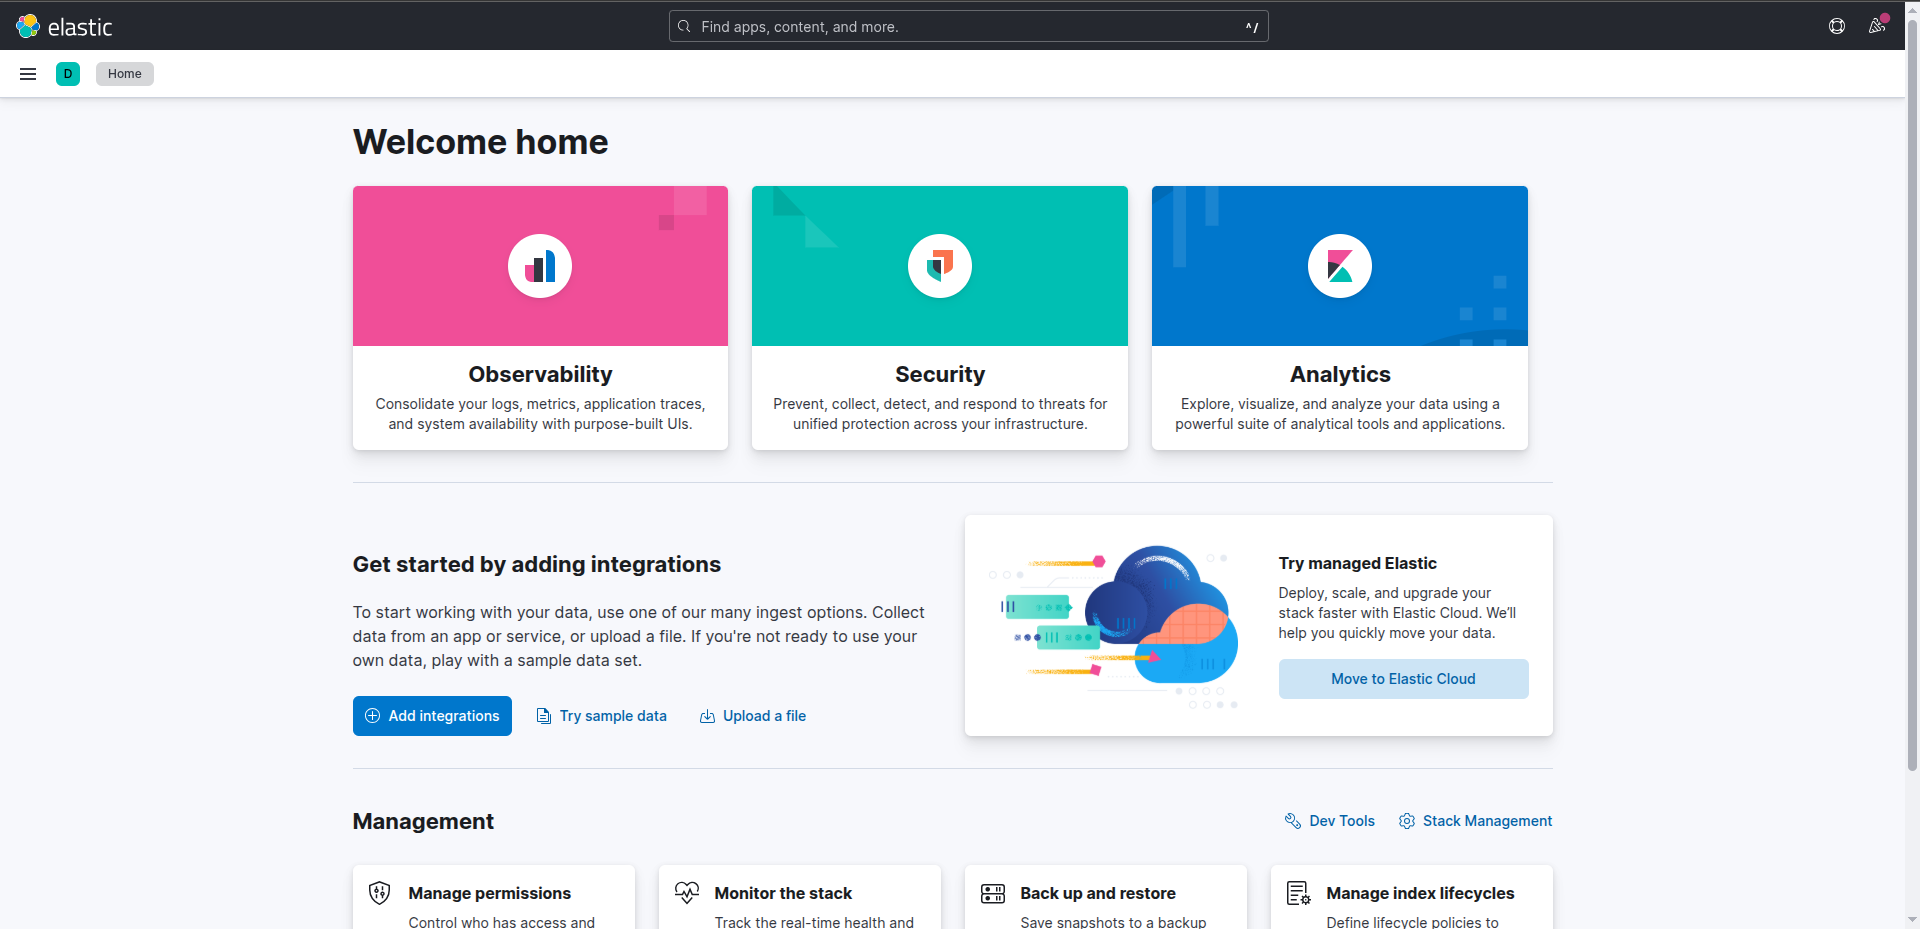
\includegraphics[width=0.90\linewidth,keepaspectratio]{screenshots/elk-browser.png}}}
  \caption{Interface Kibana 8.13 -- page d'accueil}\label{fig:elk-browser}
\end{figure}

\begin{figure}[H]
  \centering
  {\setlength{\fboxsep}{3pt}\setlength{\fboxrule}{0.4pt}
  \fbox{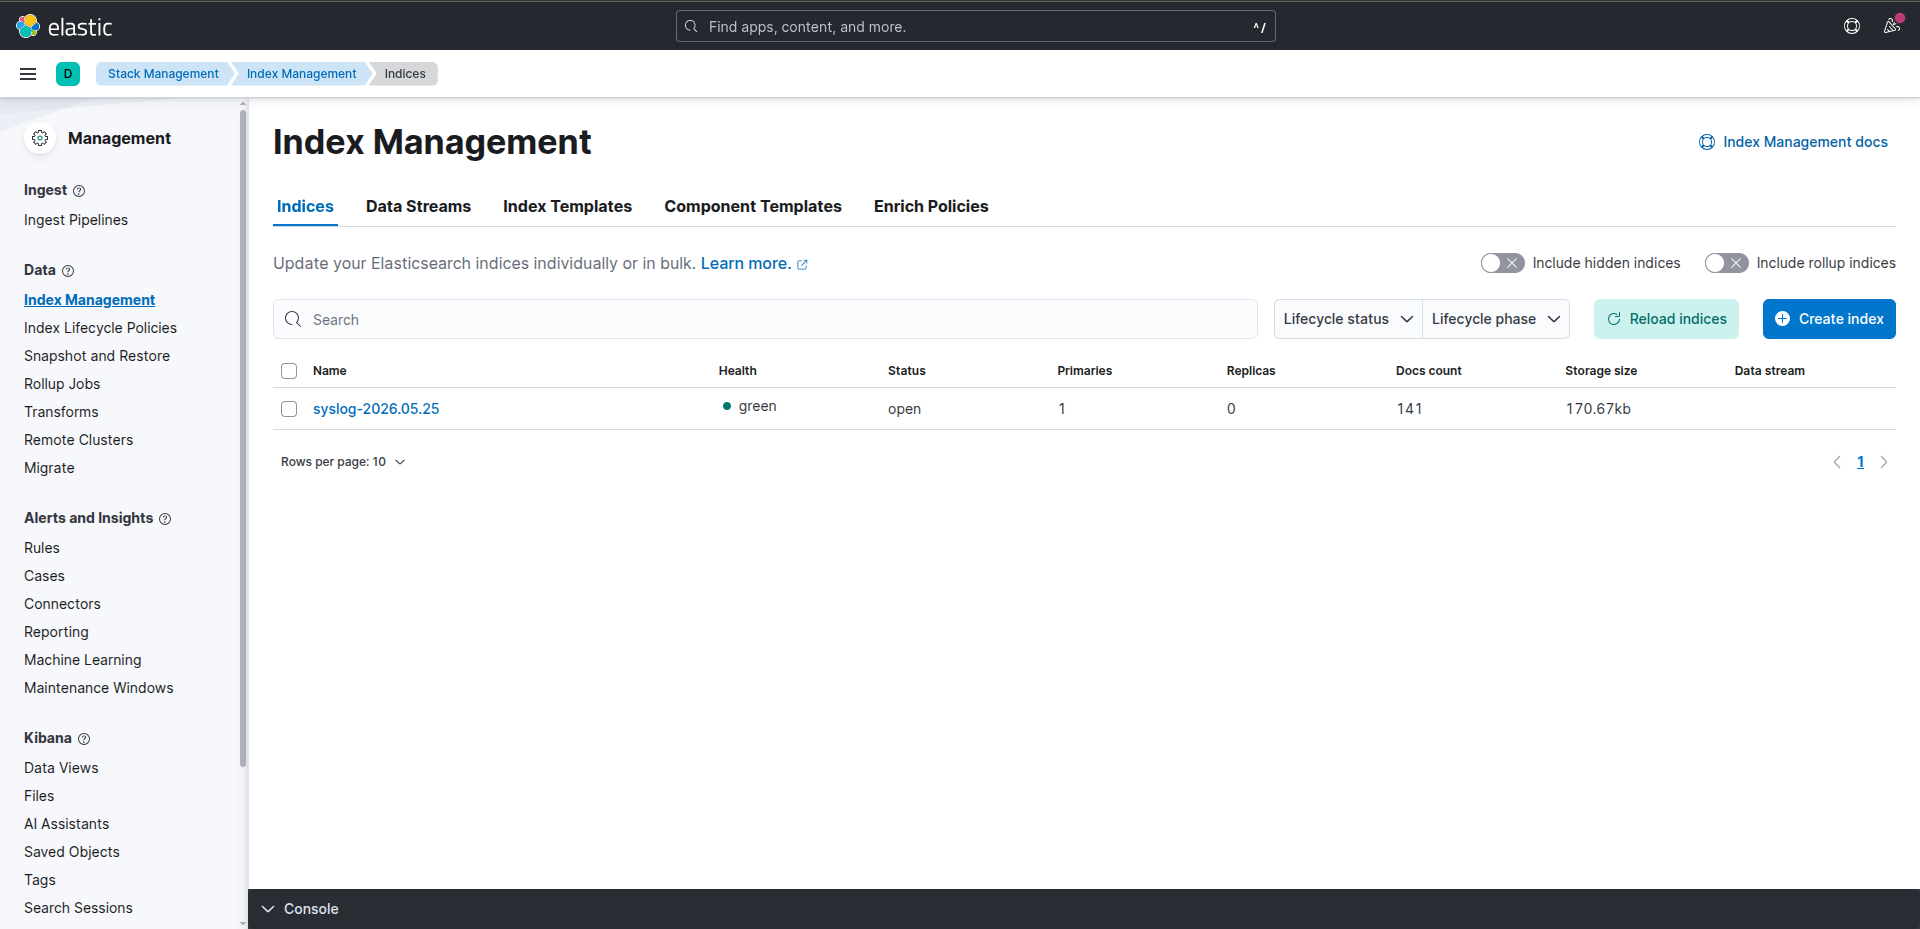
\includegraphics[width=0.90\linewidth,keepaspectratio]{screenshots/elk-index-management.png}}}
  \caption{Index \texttt{syslog-2026.05.25} -- statut green, 141 documents}\label{fig:elk-index}
\end{figure}

\begin{figure}[H]
  \centering
  {\setlength{\fboxsep}{3pt}\setlength{\fboxrule}{0.4pt}
  \fbox{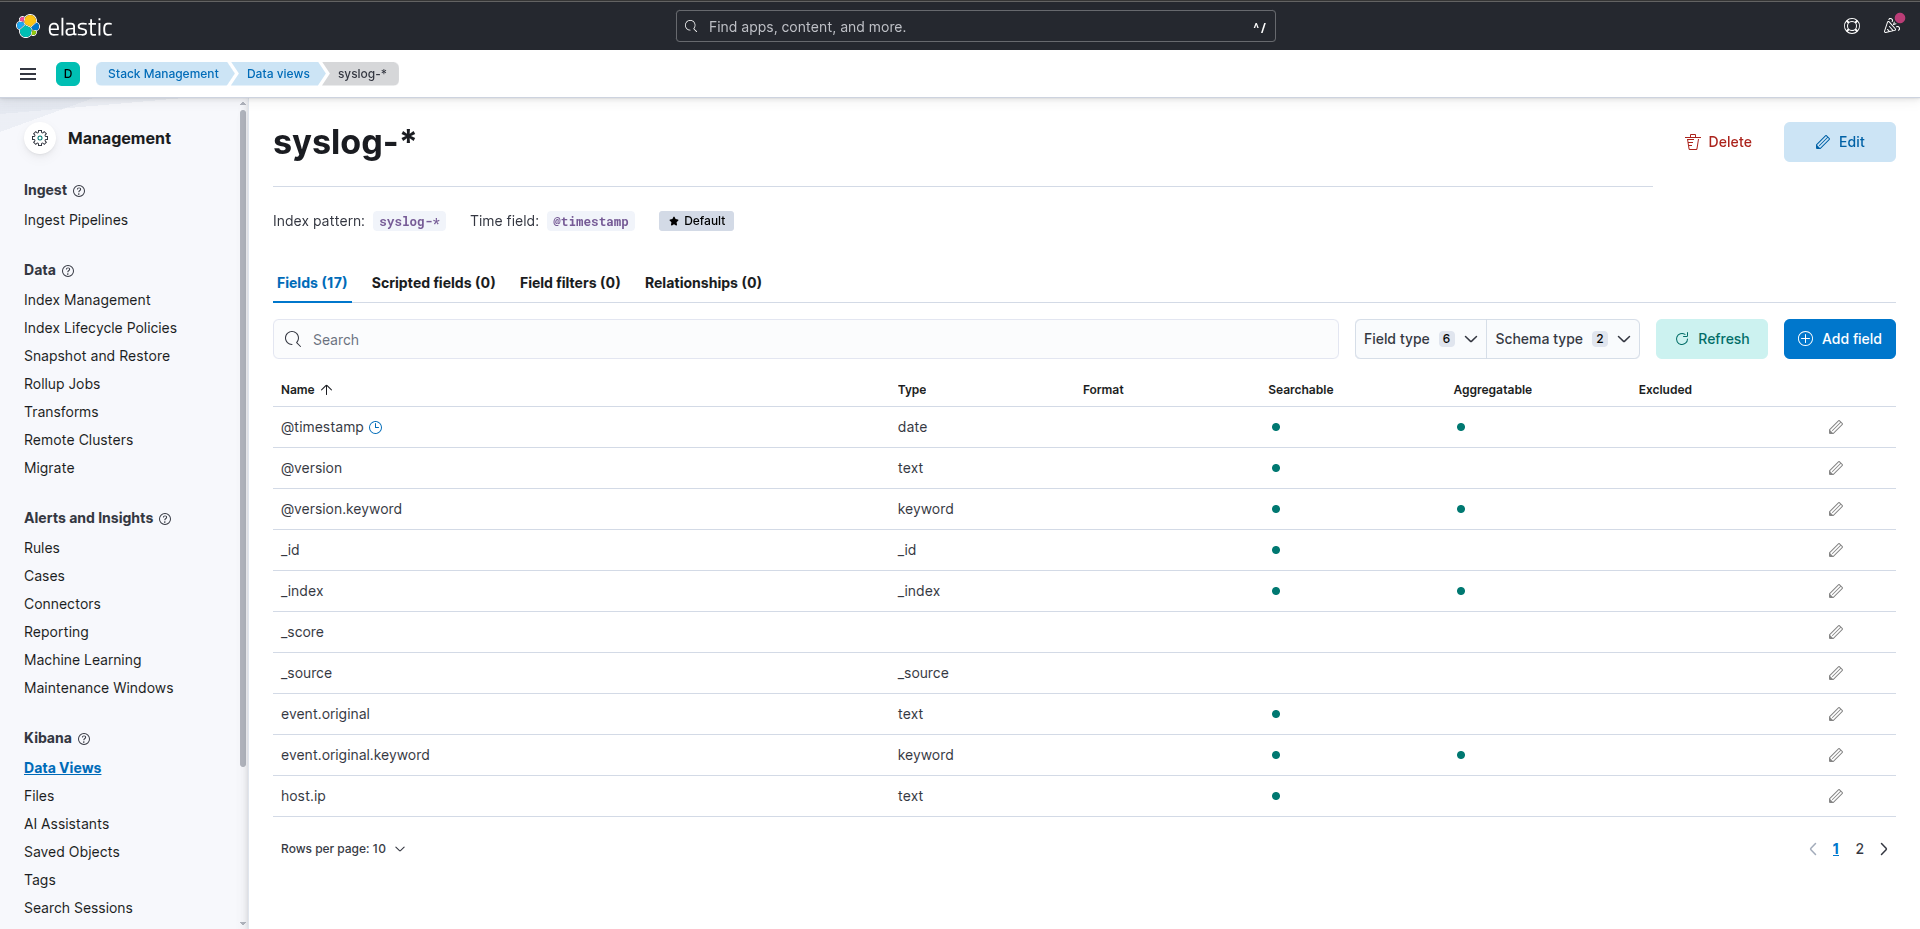
\includegraphics[width=0.90\linewidth,keepaspectratio]{screenshots/elk-data-view.png}}}
  \caption{Data view \texttt{syslog-*} avec champ temporel \texttt{@timestamp}}\label{fig:elk-dataview}
\end{figure}

\begin{figure}[H]
  \centering
  {\setlength{\fboxsep}{3pt}\setlength{\fboxrule}{0.4pt}
  \fbox{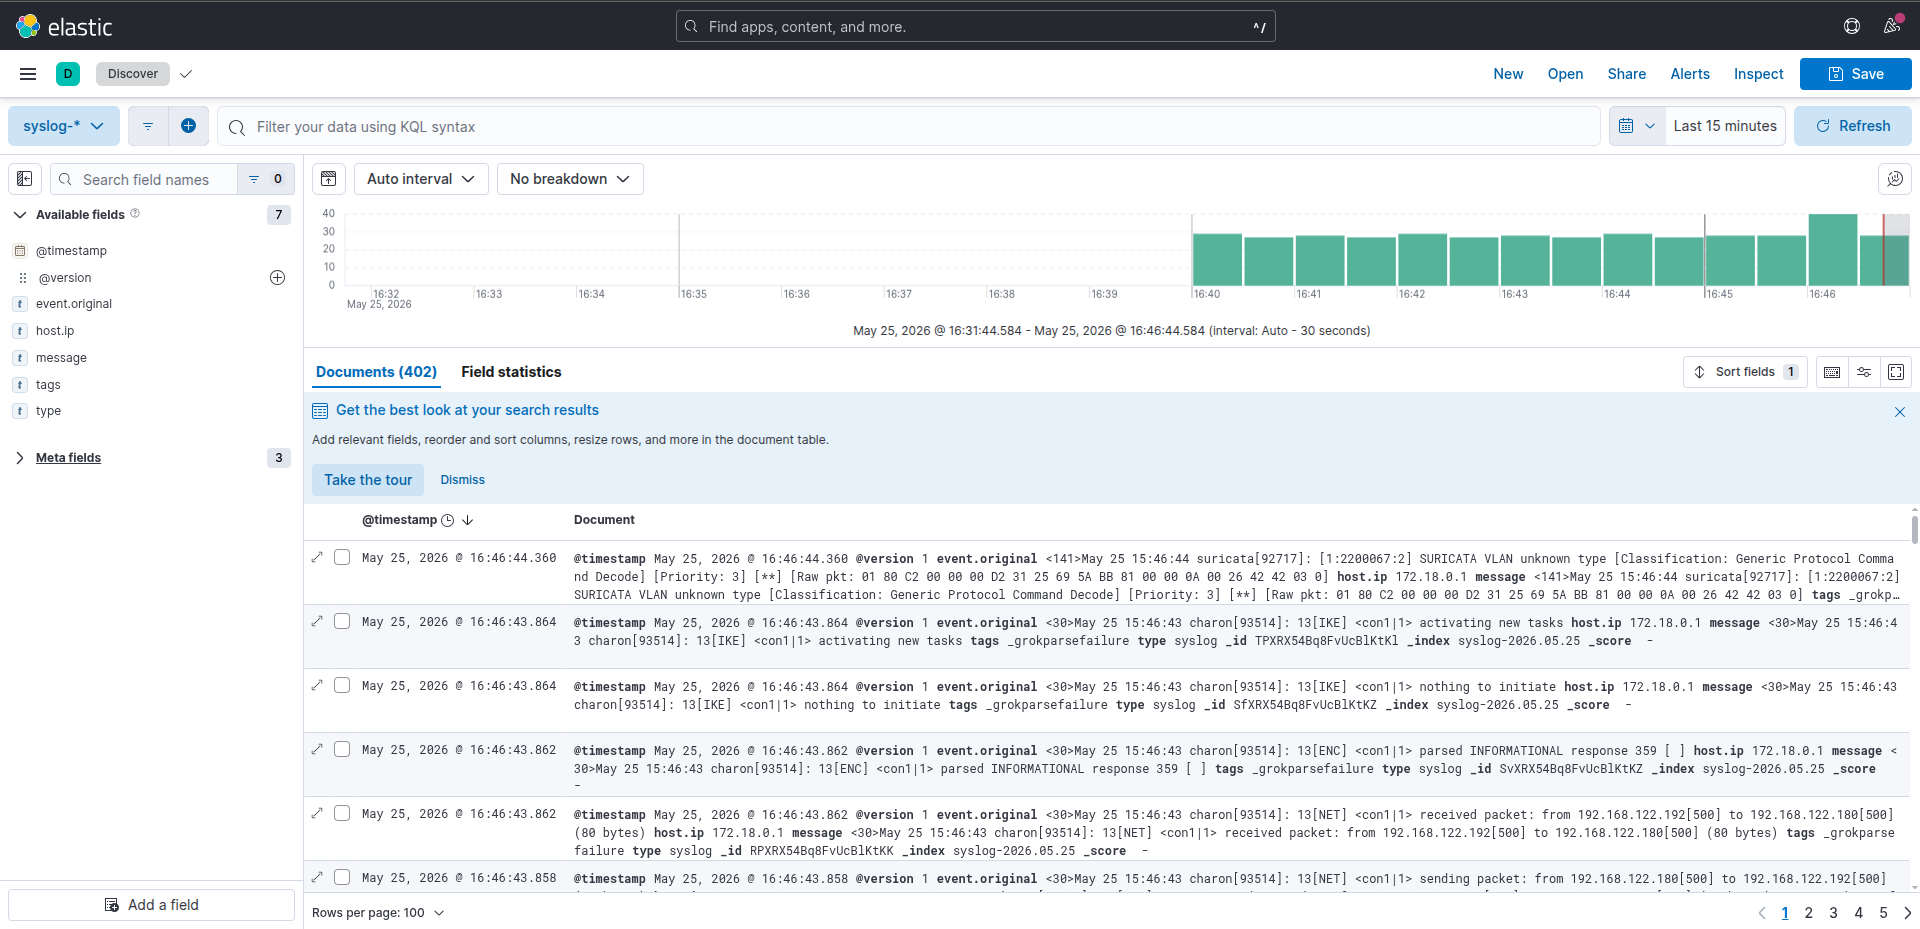
\includegraphics[width=0.90\linewidth,keepaspectratio]{screenshots/elk-discover.png}}}
  \caption{Kibana Discover -- 402 evenements pfSense dont alertes Suricata en temps reel}\label{fig:elk-discover}
\end{figure}

Les journaux visibles incluent les alertes Suricata, les evenements IPSec/IKE du tunnel VPN, et les evenements systeme pfSense. Exemple d'alerte Suricata reelle capturee dans Kibana Discover :

\begin{lstlisting}[caption={Exemple d'alerte Suricata capturee dans ELK (25 mai 2026)}]
TIMESTAMP : 2026-05-25T16:38:30.081905415Z
SOURCE    : 192.168.122.180 (pfSense-Siege WAN)
MESSAGE   : suricata[92717]: [1:2200067:2] SURICATA VLAN unknown type
            [Classification: Generic Protocol Command Decode]
            [Priority: 3]
            [Raw pkt: 01 80 C2 00 00 00 D2 31 25 69 5A BB 81 00 00 0A...]

# Verification de l'index dans Elasticsearch
$ curl -s localhost:9200/_cat/indices?v
health status index              pri rep docs.count
green  open   syslog-2026.05.25    1   0        402
\end{lstlisting}

\begin{tcolorbox}[colback=softbg,colframe=primary,title={\small\bfseries Interpretation de l'alerte},fonttitle=\color{white}]
La regle \texttt{1:2200067:2} (ETOpen) detecte des trames VLAN avec un type EtherType inconnu -- comportement normal du switch virtuel GNS3. Cette alerte de \textbf{Priorite 3} (faible) confirme que Suricata analyse bien le trafic reseau. Les alertes de priorite 1 et 2 (tentatives d'intrusion reelles) apparaitraient de la meme facon dans Kibana, avec le champ \texttt{suricata.event\_type = alert}.
\end{tcolorbox}

Cette integration ELK+Suricata constitue un SIEM leger adapte a la taille de l'infrastructure, permettant la correlation d'evenements entre le pare-feu, les serveurs et l'IDS en temps reel.

% ═════════════════════════════════════════════════════════════════════
\section{Script d'automatisation du durcissement (Bonus)}
\label{sec:script}
% ═════════════════════════════════════════════════════════════════════

Un script shell \texttt{harden\_server.sh} (452 lignes) a ete developpe pour automatiser l'ensemble des operations de durcissement documentees dans les Parties 3, 4 et 5. Ce script est idempotent dans la mesure du possible et s'execute en une seule commande sur un serveur Debian 12 fraichement installe.

\begin{lstlisting}[caption={Utilisation du script}]
# Transfert vers le serveur cible (via telnet console GNS3)
cat > /root/harden_server.sh << 'ENDSCRIPT'
  [contenu du script]
ENDSCRIPT
chmod +x /root/harden_server.sh
bash /root/harden_server.sh
\end{lstlisting}

Le script est structure en sections correspondant aux parties du mini-projet :

\begin{table}[H]
\centering
\begin{tabular}{@{}lll@{}}
\toprule
\textbf{Section} & \textbf{Partie} & \textbf{Operations} \\
\midrule
{[3.1]} & Systeme & \texttt{apt upgrade}, unattended-upgrades, chrony, services desactives \\
{[3.2]} & SSH & sshd\_config complet, banniere, generation cle RSA 4096 \\
{[3.3]} & UFW & reset, politique deny, regles par role serveur \\
{[3.4]} & Services & Apache+SSL, MariaDB securise, OpenLDAP+OUs+users \\
{[4.2]} & IAM & pam\_pwquality, pam\_google\_authenticator, limites PAM \\
{[4.3]} & Sudo & suppression comptes inutiles, sudoers granulaire \\
{[5.1]} & Logs & rsyslog transfert centralise \\
{[5.2]} & IDS & fail2ban jail.local complet \\
{[5.3]} & Integrite & rkhunter propupd, aide --init, cron hebdomadaire \\
{[5.4]} & Backup & script GPG AES-256, cron quotidien 2h00 \\
\bottomrule
\end{tabular}
\caption{Structure du script harden\_server.sh}
\label{tab:script}
\end{table}

Des scripts specifiques par serveur (\texttt{harden\_fichiers.sh}, \texttt{harden\_web.sh}, \texttt{harden\_mail.sh}) adaptent les regles UFW et les services installes au role de chaque machine. Un script Python (\texttt{upload\_harden\_mp2.py}) automatise le transfert via telnet vers les consoles GNS3.

% ═════════════════════════════════════════════════════════════════════
\section{Tests de securite}
% ═════════════════════════════════════════════════════════════════════

Configurer n'est pas suffisant -- il faut verifier que la configuration produit bien le comportement attendu. Notre approche de test a ete systematique : pour chaque mecanisme de securite deploye, nous avons execute un test qui le valide en conditions reelles. Les resultats presentes ici sont des sorties reelles capturees dans l'environnement GNS3, pas des simulations.

\subsection{Verification des regles UFW}

Apres activation d'UFW sur chaque serveur, la commande \texttt{ufw status numbered} confirme les regles actives. La capture suivante montre les 7 regles definitives sur le serveur Fichiers apres suppression des regles temporaires de test :

\begin{figure}[H]
  \centering
  {\setlength{\fboxsep}{3pt}\setlength{\fboxrule}{0.4pt}
  \fbox{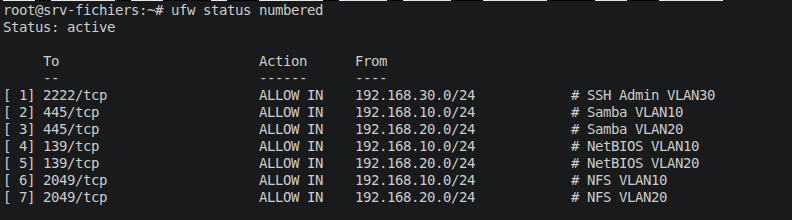
\includegraphics[width=0.90\linewidth,keepaspectratio]{real-results/firewall-rules-example.png}}}
  \caption{UFW status numbered sur srv-fichiers -- 7 regles de production (Samba, NFS, SSH VLAN30)}\label{fig:ufw-rules-fichiers}
\end{figure}

Exemple sur AD-LDAP (\texttt{ufw status verbose}) :

\begin{lstlisting}[caption={Statut UFW sur AD-LDAP apres durcissement}]
Status: active
Default: deny (incoming), allow (outgoing)

To                         Action      From
--                         ------      ----
2222/tcp                   ALLOW IN    192.168.30.0/24  # SSH Admin
80/tcp                     ALLOW IN    Anywhere         # HTTP
443/tcp                    ALLOW IN    Anywhere         # HTTPS
389/tcp                    ALLOW IN    192.168.10.0/24  # LDAP
636/tcp                    ALLOW IN    192.168.10.0/24  # LDAPS
3306/tcp                   ALLOW IN    192.168.10.0/24  # MariaDB
3306/tcp                   ALLOW IN    192.168.20.0/24  # MariaDB VLAN20
\end{lstlisting}

\subsection{Verification de la securisation MariaDB}

Apres application des commandes de securisation sur le conteneur Docker BDD-MariaDB :

\begin{lstlisting}[caption={Verification des comptes MariaDB apres securisation}]
MariaDB> SELECT user, host FROM mysql.user;
+-------------+-----------+
| user        | host      |
+-------------+-----------+
| healthcheck | 127.0.0.1 |
| healthcheck | ::1       |
| healthcheck | localhost |
| mariadb.sys | localhost |
| root        | localhost |  <- seul root@localhost reste
+-------------+-----------+
\end{lstlisting}

Le compte \texttt{root@\%} (acces depuis n'importe quelle IP) a ete supprime. La base \texttt{test} a ete supprimee.

\subsection{Verification du tunnel VPN}

Le statut du tunnel IPSec dans pfSense confirme l'etablissement des deux phases. La connectivite a ete testee par ping entre les deux sites via le tunnel chiffre (voir figure~\ref{fig:pfsense-vpn-ok}).

\subsection{Verification LDAP}

L'annuaire a ete verifie par une recherche LDAP apres creation des OUs et comptes :

\begin{lstlisting}[caption={Sortie reelle -- ldapsearch sur AD-LDAP}]
$ ldapsearch -x -H ldap://localhost \
    -D "cn=admin,dc=mobitech,dc=local" -w "Mobitech2024!" \
    -b "dc=mobitech,dc=local" "(objectClass=organizationalUnit)" dn

# LDAPv3  base: dc=mobitech,dc=local

dn: ou=Direction,dc=mobitech,dc=local
dn: ou=RH,dc=mobitech,dc=local
dn: ou=IT,dc=mobitech,dc=local
dn: ou=Commercial,dc=mobitech,dc=local

# numEntries: 4

$ slapcat -n 1 | grep "^dn:"
dn: dc=mobitech,dc=local
dn: ou=Direction,dc=mobitech,dc=local
dn: ou=RH,dc=mobitech,dc=local
dn: ou=IT,dc=mobitech,dc=local
dn: ou=Commercial,dc=mobitech,dc=local
dn: uid=adminit,ou=IT,dc=mobitech,dc=local
dn: uid=directeur,ou=Direction,dc=mobitech,dc=local
\end{lstlisting}

\subsection{Test de scan de ports (Nmap)}

Un scan Nmap a ete realise depuis la machine hote (representant un poste hors VLAN30) sur le serveur AD-LDAP (192.168.122.52) :

\begin{lstlisting}[caption={Scan Nmap sur AD-LDAP -- resultat reel}]
$ sudo nmap -sS --open -p 22,2222,80,443,389,636,3306 192.168.122.52

Nmap scan report for 192.168.122.52
Host is up (0.011s latency).
Not shown: 5 filtered tcp ports (no-response)

PORT    STATE  SERVICE
80/tcp  open   http
443/tcp open   https

# Ports 22, 2222, 389, 636, 3306 -> filtered (UFW bloque)
\end{lstlisting}

Interpretation :
\begin{itemize}[noitemsep,leftmargin=1.4em]
  \item \textbf{80/443 ouverts} : normal pour le serveur AD-LDAP (Apache).
  \item \textbf{2222 (SSH) filtre} : la machine hote n'est pas dans 192.168.30.0/24, UFW bloque.
  \item \textbf{389/636 (LDAP/LDAPS) filtres} : protege au niveau VLAN10 uniquement.
  \item \textbf{3306 (MariaDB) filtre} : bind sur 192.168.10.10, inaccessible depuis l'exterieur.
\end{itemize}

\subsection{Test de brute-force SSH et fail2ban}

fail2ban a ete teste en autorisant temporairement SSH depuis la machine hote (192.168.122.0/24) via une regle UFW de test, puis en envoyant 7 tentatives SSH avec un utilisateur invalide :

\begin{lstlisting}[caption={Test fail2ban -- resultat reel}]
# Ajout regle UFW temporaire pour le test
ufw allow from 192.168.122.0/24 to any port 2222 proto tcp

# 7 tentatives SSH avec utilisateur inexistant
for i in $(seq 1 7); do
    ssh -p 2222 -o BatchMode=yes baduser@192.168.122.52; done

# Verification du ban (sur AD-LDAP) :
$ fail2ban-client status sshd
Status for the jail: sshd
|- Filter
|  |- Currently failed: 1
|  |- Total failed:     7
`- Actions
   |- Currently banned: 1
   `- Banned IP list:   192.168.122.1   <- hote banni
\end{lstlisting}

\begin{figure}[H]
  \centering
  {\setlength{\fboxsep}{3pt}\setlength{\fboxrule}{0.4pt}
  \fbox{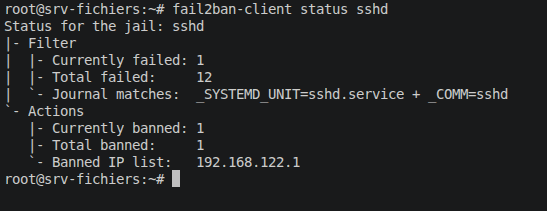
\includegraphics[width=0.90\linewidth,keepaspectratio]{real-results/fail2ban.png}}}
  \caption{fail2ban -- IP 192.168.122.1 bannie apres 6 tentatives SSH echouees}\label{fig:fail2ban-ban}
\end{figure}

\begin{figure}[H]
  \centering
  {\setlength{\fboxsep}{3pt}\setlength{\fboxrule}{0.4pt}
  \fbox{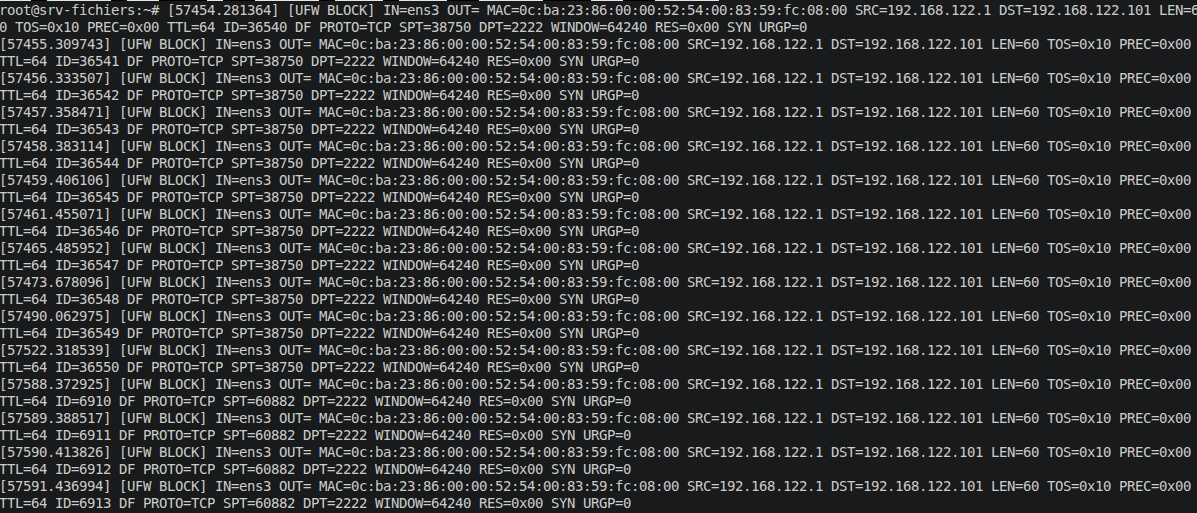
\includegraphics[width=0.90\linewidth,keepaspectratio]{real-results/ufw-block.png}}}
  \caption{UFW bloquant en temps reel les tentatives SSH depuis un hote non autorise (192.168.122.1)}\label{fig:ufw-block}
\end{figure}

\begin{tcolorbox}[colback=primarylight,colframe=primary!40,arc=4pt,boxrule=0.6pt,
  left=8pt,right=8pt,top=6pt,bottom=6pt]
\textbf{Double couche de protection :} UFW bloque les connexions SSH depuis les IPs hors VLAN30 avant qu'elles atteignent sshd (filtrage reseau en amont). L'attaquant ne recoit meme pas de reponse TCP. fail2ban intervient comme deuxieme couche pour les IPs autorisees par UFW qui font du brute-force -- les deux mecanismes sont complementaires.
\end{tcolorbox}

Apres le test, la regle UFW temporaire a ete supprimee et l'IP debannee (\texttt{fail2ban-client set sshd unbanip 192.168.122.1}).

% ═════════════════════════════════════════════════════════════════════
\section{Bilan et perspectives}
% ═════════════════════════════════════════════════════════════════════

\subsection{Ce qui a ete realise}

\begin{table}[H]
\centering
\begin{tabular}{@{}p{7cm}lp{5cm}@{}}
\toprule
\textbf{Objectif} & \textbf{Statut} & \textbf{Note} \\
\midrule
Topologie GNS3 avec VLANs 10/20/30 et DMZ & \textcolor{okgreen}{\textbf{Realise}} & \\
pfSense CE 2.8.1 installe et configure & \textcolor{okgreen}{\textbf{Realise}} & \\
Regles pare-feu par zone & \textcolor{okgreen}{\textbf{Realise}} & \\
NAT sortant Hybrid mode & \textcolor{okgreen}{\textbf{Realise}} & \\
VPN IPSec IKEv2 AES-256 site-a-site & \textcolor{okgreen}{\textbf{Realise}} & Tunnel etabli \\
SSH durci (port 2222, cle+MFA) & \textcolor{okgreen}{\textbf{Realise}} & Sur QEMU VMs \\
UFW par role serveur & \textcolor{okgreen}{\textbf{Realise}} & \\
Apache HTTPS + headers securite & \textcolor{okgreen}{\textbf{Realise}} & \\
MariaDB securise (Docker + QEMU) & \textcolor{okgreen}{\textbf{Realise}} & \\
OpenLDAP mobitech.local + OUs & \textcolor{okgreen}{\textbf{Realise}} & \\
pam\_pwquality (complexite MDP) & \textcolor{okgreen}{\textbf{Realise}} & \\
MFA Google Authenticator SSH & \textcolor{okgreen}{\textbf{Realise}} & Config PAM deployee \\
Sudo granulaire par groupe & \textcolor{okgreen}{\textbf{Realise}} & \\
rsyslog centralise vers AD-LDAP & \textcolor{okgreen}{\textbf{Realise}} & \\
fail2ban (SSH, HTTP, mail) & \textcolor{okgreen}{\textbf{Realise}} & \\
rkhunter + aide baseline & \textcolor{okgreen}{\textbf{Realise}} & \\
Sauvegarde GPG AES-256 quotidienne & \textcolor{okgreen}{\textbf{Realise}} & \\
Script d'automatisation (bonus) & \textcolor{okgreen}{\textbf{Realise}} & harden\_server.sh 452 lignes \\
IDS Suricata 7.0.11 (LAN+WAN) & \textcolor{okgreen}{\textbf{Realise}} & ETOpen rules, EVE JSON, mode passif \\
Stack ELK 8.13 (bonus) & \textcolor{okgreen}{\textbf{Realise}} & 402 evenements pfSense+Suricata indexes \\
SSSD integration postes VLAN20 & \textcolor{warnred}{\textbf{Partiel}} & Schema posixAccount pret, VPCS sans OS Linux \\
\bottomrule
\end{tabular}
\caption{Bilan des realisations}
\label{tab:bilan}
\end{table}

\subsection{Limites et ameliorations envisagees}

\textbf{IDS/IPS en mode IPS} : Suricata est actuellement en mode IDS passif (detection seule). Le passage en mode IPS inline (blocage actif) sur pfSense necessite de basculer en mode \textit{Workers} et d'activer \textit{Block Offenders}, ce qui peut impacter les performances dans un environnement de production.

\textbf{Certificats TLS valides} : Les certificats auto-signes actuels genereront des alertes navigateur en production. Le deploiement d'une PKI interne (par exemple avec \texttt{step-ca}) ou l'integration de Let's Encrypt (si les serveurs sont accessibles depuis Internet) est recommande.

\textbf{SSSD / integration LDAP-PAM} : Les postes VLAN20 sont des noeuds VPCS dans GNS3 (pas d'OS Linux complet). Le schema LDAP \texttt{posixAccount} est en place ; l'integration SSSD sera possible des que les postes seront migres vers des VMs Debian/Ubuntu.

\textbf{Supervision reseau} : Un outil de supervision (Zabbix, Prometheus+Grafana) permettrait de surveiller la disponibilite des services, la charge CPU/RAM des serveurs et les metriques reseau en temps reel.

\textbf{Chiffrement LDAP} : Le service slapd ecoute actuellement sur le port 389 (LDAP en clair). La migration vers LDAPS (port 636) avec un certificat TLS doit etre realisee pour chiffrer les echanges d'annuaire sur le reseau.

% ─────────────────────────────────────────────────────────────────────
\vspace{1.5em}
\begin{tcolorbox}[colback=primarylight,colframe=primary,arc=5pt,boxrule=0.8pt,
  left=10pt,right=10pt,top=8pt,bottom=8pt]
\textbf{Conclusion.} Ce mini-projet nous a permis de concevoir et de deployer de bout en bout une infrastructure reseau d'entreprise realiste, en partant d'un reseau plat non segmente pour arriver a une architecture multi-zones securisee avec pare-feu, VPN site-a-site, annuaire centralise et surveillance active. Nous avons fait le choix de privilegier des outils open-source eprouvees -- pfSense, OpenLDAP, Suricata, ELK -- afin de rester au plus pres des pratiques rencontrees en production. Les perspectives d'evolution portent sur le passage de Suricata en mode IPS inline, le deploiement d'une PKI interne, et l'integration SSSD sur les postes employes pour une authentification entierement centralisee.
\end{tcolorbox}

\end{document}
